% =====================================================================
% EXTp: A Soundness Theorem for Counterfactual Exploit Replay on
% Formally Verified Microkernels
%
% NDSS 2028 Fall Cycle submission
% Deadline: NDSS 2028 cycle (TBD)
% Target: 13 pp main body, 18 pp camera-ready (double-column)
%
% CLASS SELECTION ----------------------------------------------------
% To compile with the official NDSS template:
%   1. Download the NDSS 2026 template zip from
%      https://www.ndss-symposium.org/ndss2026/submissions/templates/
%   2. Upload ndss.cls (and any auxiliary files) to this Overleaf project
%   3. Use:  \documentclass[conference]{ndss}
%
% For preview/early drafting without ndss.cls, use IEEEtran (geometry
% is close but not exact; switch to ndss.cls before final submission).
% =====================================================================

% --- ACTIVE CLASS (swap when ndss.cls is uploaded) ---
\documentclass[conference]{IEEEtran}
% \documentclass[conference]{ndss}  % NOT NEEDED: NDSS official template (bare_conf_NDSS2028) IS IEEEtran[conference]

% --- PACKAGES (work with both classes) ---
\usepackage[T1]{fontenc}
\usepackage[utf8]{inputenc}
\usepackage{amsmath}
\usepackage{amssymb}
\usepackage{amsthm}
\usepackage{mathtools}
\usepackage{booktabs}
\usepackage{enumitem}
\usepackage{xcolor}
\usepackage{graphicx}
\usepackage{tikz}
\usetikzlibrary{arrows.meta, positioning, fit, calc, shapes.geometric}
\usepackage{hyperref}
\usepackage{cleveref}

% --- THEOREM ENVIRONMENTS ---
\newtheorem{theorem}{Theorem}
\newtheorem{proposition}{Proposition}
\newtheorem{lemma}{Lemma}

% --- CUSTOM COMMANDS ---
\newcommand{\Korig}{T_\text{orig}}
\newcommand{\Tcf}{T_\text{cf}}
\newcommand{\Kverified}{\mathcal{K}_\text{verified}}
\newcommand{\Kextended}{\mathcal{K}_\text{extended}}
\newcommand{\Kint}{\mathcal{K}_\text{int}}
\newcommand{\Kfwk}{\mathcal{K}_\text{fwk}}
\newcommand{\sigbase}{\hat{\sigma}_\text{baseline}}
\newcommand{\Dstar}{\Delta^{*}}
\newcommand{\arealized}{\alpha_\text{realized}}
\newcommand{\scoreS}{\text{score}_S}
\newcommand{\dox}[1]{\text{do}(X{=}#1)}
\newcommand{\epsSOE}{\varepsilon_\text{SOE}}

% --- ARTIFACT URL (Isabelle development, measurement data, boot images) ---
\newcommand{\artifacturl}{https://github.com/heavyisthecrown0x11/extp-artifact}

% --- HYPHENATION (minor cleanup for narrow columns) ---
\hyphenation{counter-factual micro-architectural hyper-visor}

% =====================================================================
\begin{document}

\title{EXTp: A Soundness Theorem for Counterfactual Exploit Replay on Formally Verified Microkernels}

% --- AUTHOR BLOCK (camera-ready; anonymous block removed 2026-09-09) ---
\author{\IEEEauthorblockN{Utku Erol}\\
\IEEEauthorblockA{\textit{Independent Researcher}\\
\texttt{utkuerol71@gmail.com}}}

\maketitle

% =====================================================================
\begin{abstract}
Counterfactual exploit analysis --- determining which input
parameter causally produced an observed outcome --- is pervasive
in security research, but its current practice is epistemically
unsound. Three gaps separate ``different outcome'' from ``caused
by the change'': non-deterministic replay noise, replay-machinery
side-effects, and causal pathways traversing microarchitectural
state invisible to the analyst's surface. We present EXTp, a
counterfactual replay framework on bare-metal seL4, and the
Counterfactual Soundness Theorem (CST) --- the first formal
soundness theorem for counterfactual causal attribution grounded
in a verified microkernel substrate. EXTp realizes three
observable properties: Capability
Separation (Pearl modularity; Clopper-Pearson bound
${\leq}0.37\%$ at $N{=}998$), Strong Observational Equivalence
(replay determinism: $\scoreS{=}1.0000$ observed over $N{=}34$
cross-boot trials, Clopper-Pearson one-sided $95\%$ upper bound on
the per-run failure rate ${\leq}10.4\%$), and Measurement
Interference (calibrated timing threshold,
realized false-positive rate $0.61\%$--$2.78\%$). CST proves their
composition grounds Pearl/Halpern-Pearl causal attribution within
enumerated epistemic bounds; CST v1.0 establishes soundness under
single-VCPU intervention scope and bare-metal microcode-stable
configurations, with multi-VCPU and cross-configuration extensions
charted as future work. A synthetic analog modeled on the
CrackArmor confused-deputy pattern, executed on bare-metal Intel
Alder Lake, exercises the pipeline end-to-end and shows the
framework correctly detecting its own A1-modulo violations.
\end{abstract}

% =====================================================================
\section{Introduction}\label{sec:intro}

Determining \emph{why} an exploit succeeds is harder than determining
\emph{that} it succeeds. A crash, a privilege escalation, a sandbox
escape --- these are observable. Whether a specific input parameter
\emph{caused} the outcome, or whether a different parameter value
would have prevented it, is a counterfactual question. Current
practice answers it informally: re-run with a modified input, observe
whether the outcome changes, call it causal. This methodology is
pervasive, and it is epistemically unsound. Three gaps separate
``different outcome'' from ``caused by the change'':
non-deterministic replay noise that can mimic causal signals; replay
machinery side-effects that confound the measurement; and causal
pathways that traverse microarchitectural state invisible to the
analyst's observable surface. Without formal guarantees addressing
all three, counterfactual exploit analysis is intuition dressed as
method.

The theoretical machinery to close these gaps exists. Pearl's
structural causal model~\cite{pearl2009causality} defines the
$\dox{x'}$ intervention operator and the axioms --- modularity,
faithfulness, effectiveness --- that make causal attribution provably
sound. Halpern and Pearl's actual-causation
conditions~\cite{halpern2005causes} specify precisely when an
observed outcome is attributable to a named cause. Yet this apparatus
has not been applied to exploit analysis. The obstacle is structural:
Pearl's framework is probabilistic and abstract, defined over
distributions and idealized structural equations. Exploit replay
operates on concrete microarchitectural traces --- TSC measurements
with asymmetric noise floors, VM-exit surfaces with finite register
coverage, capability-mediated VMM machinery with empirical rather
than axiomatic side-effect bounds. To our knowledge, no prior work
formally bridges this gap.

We present \textbf{EXTp}, and with it the \textbf{first soundness
theorem for counterfactual causal attribution in exploit analysis
grounded in a formally verified substrate}. Prior Pearl-applied
work in adjacent domains~\cite{fariha2020aid} (AID, SIGMOD 2020)
demonstrates probabilistic causal attribution for database failures
but does not provide a soundness theorem grounded in a verified
computational base; conceptual extensions of the HP
framework~\cite{soloviev2021nested} provide no operational system.
CST is the first theorem-grade formalization of admissibility
under enumerated antecedents on a verified substrate. EXTp is a
counterfactual replay framework on a bare-metal
seL4~\cite{klein2009sel4} virtual machine monitor. Its Counterfactual
Soundness Theorem (CST) proves that, under the formal assumptions
grounded in EXTp's observable properties, replay-based causal
attribution satisfies Pearl's effectiveness and composition axioms
(modularity realized by CapSep, faithfulness subsumed by SOE) and
Halpern-Pearl's AC1 and AC2 actual-causation conditions --- with
divergence points (irreversibility inapplicable; determinism strictly
stronger than faithfulness) declared explicitly rather than elided.
The result is a system where ``$\dox{x'}$ caused divergence $D$ at
event $i$'' is not an analyst's intuition but a formally admissible
claim within an enumerated epistemic envelope.

EXTp achieves this through three observable properties that compose
into CST. \textbf{Capability Separation (CapSep)} proves intervention
authority disjointness ($\Kint \cap \Kfwk = \emptyset$), realizing
Pearl's modularity axiom: $\dox{x'}$ cannot directly modify
framework-internal state. For seL4's formally verified operations,
this follows from seL4's Isabelle/HOL proof harness; for extended
VT-x operations, it is empirically bounded with Clopper-Pearson
confidence. \textbf{Strong Observational Equivalence (SOE)}
establishes trajectory-level replay determinism
($\scoreS = 1.0000$, $N{=}34$ cross-boot trials), a property strictly
stronger than Pearl's probabilistic faithfulness and sufficient to
rule out coincidence as an alternative explanation for observed
divergence. \textbf{Measurement Interference (MI)} derives a
calibrated timing detection threshold $\Dstar = z_{1-\alpha} \cdot
\sigbase$ with empirically realized false-positive rate
$0.61\%$--$2.78\%$, bounding the residual confounding that CapSep
does not eliminate. CST proves that together these three properties
are sufficient to ground Pearl-style causal attribution within an
explicitly enumerated epistemic envelope.

This paper makes four contributions.
\textbf{(C1)} EXTp: a counterfactual exploit replay framework on
bare-metal seL4 with four intervention classes and cross-boot replay
stability $\scoreS = 1.0000$ over $N{=}34$ trials.
\textbf{(C2)} Three independently verifiable observable properties
--- CapSep (modularity axiom), SOE (faithfulness/determinism), MI
(confounder boundedness) --- each making falsifiable claims about a
distinct dimension of the replay machinery.
\textbf{(C3)} CST: the first formal soundness theorem for
counterfactual causal attribution in exploit analysis, with explicit
Pearl/Halpern-Pearl correspondence, declared divergence points, and a
proof whose \emph{conditional core} --- the composition of the
antecedent envelope $(A_1, A_2, A_3, A_4)$ into the Pearl/Halpern-Pearl
correspondence properties --- is machine-checked in Isabelle/HOL, with
the empirical antecedents calibration-supplied and the seL4 lifting
left to future work (\S\ref{sec:discussion-isabelle}).
\textbf{(C4)} A privilege-check-bypass demonstration modeled on the
CrackArmor confused-deputy exploit pattern\footnote{The AppArmor
confused-deputy cluster (9 CVEs); analyzed using EXTp's vault
infrastructure. Chronomaly (CVE-2025-38352, POSIX CPU timer UAF) is
a scope boundary example, not a demonstration target; see \S3 Out of
Scope, item~1.} on bare-metal seL4 showing an end-to-end
CST-admissible causal attribution from a forged capability token to
an observable VM-exit divergence.

The remainder of this paper is structured as follows. \S\ref{sec:background}
provides background on seL4, VT-x VM-exits, and Pearl causality.
\S\ref{sec:threat} defines the threat model. \S\ref{sec:framework}
describes EXTp's framework design. \S\ref{sec:properties} states and
proves the four formal properties. \S\ref{sec:eval} presents the
evaluation. \S\ref{sec:discussion} discusses scope and downstream
applications. \S\ref{sec:related} surveys related work.
\S\ref{sec:conclusion} concludes.

% =====================================================================
\section{Background}\label{sec:background}

\subsection{seL4 and the Capability Model}

seL4 is a formally verified L4 microkernel whose functional
correctness, integrity, and confidentiality properties are
mechanically proven in
Isabelle/HOL~\cite{klein2009sel4,klein2014sel4}. EXTp uses seL4 as
its VMM substrate, inheriting the proof as a trust anchor for
Capability Separation. seL4's capability model partitions authority
into unforgeable tokens: a thread may only access a resource if it
holds a capability to that resource, and capabilities are manipulated
exclusively through kernel-mediated operations.

For EXTp's purposes, two operation sets are distinguished.
$\Kverified \supseteq \{\text{create}, \text{copy}, \text{revoke},
\text{destroy}\}$ comprises the cap-table operations that fall
within seL4's L4.verified formal scope; the listed subset is
those operations directly relevant to EXTp's intervention surface,
while $\Kverified$ in full is the larger L4.verified-covered
API. Their external atomicity --- the property that state
transitions are observable as single steps from outside the
kernel --- is established by the Isabelle
proof~\cite{klein2009sel4}. $\Kextended \supseteq \{\text{MapEPT},
\text{Unmap}, \text{WriteVMCS}, \text{ReadVMCS}\}$ (full enumeration
in Appendix~\ref{app:kextended}) comprises the x86-64 VT-x extension
operations that EXTp's intervention machinery uses directly; these
lie outside L4.verified's formal scope and their atomicity properties
are empirically bounded (Clopper-Pearson $95\%$ CI $\leq 10.4\%$ at
$N{=}34$ cross-boot; the CapSep-level bound $\leq 0.37\%$ at $N{=}998$
is detailed in \S\ref{sec:capsep}). The distinction matters: CapSep's
formal guarantee for $\Kverified$ is unconditional; for $\Kextended$
it is empirically conditioned and subject to Q4 validation
(\S\ref{sec:capsep}).

\subsection{VT-x VM-exits and the Observable Surface}

Intel VT-x delivers control to the VMM on every VM-exit, populating
a VMCS exit-information field with the exit reason, exit
qualification, and guest register state. EXTp captures a 4-tuple
observable surface per VM-exit:
\begin{equation}
\begin{aligned}
\text{observable}(X) = \langle\,&\text{rip}(X),\ \text{exit\_reason}(X), \\
                                &\text{exit\_qual}(X),\ \text{rax}(X)\,\rangle
\end{aligned}
\end{equation}

This surface is intentionally narrow. Other general-purpose registers
(rbx, rcx, \ldots, r15) are captured internally but excluded from the
formal surface to maintain falsifiability --- a surface defined over
all registers would require claims about register-level determinism
that EXTp's current calibration does not support (\S\ref{sec:soe}).
The surface is sufficient for the class of exploits EXTp targets:
VM-exit-boundary privilege escalations whose causal signal manifests
in instruction-pointer divergence, exit-reason changes, or return
value modification.

\subsection{Pearl Causality and Actual Causation}

Pearl's structural causal model formalizes causation through the
$\dox{x'}$ intervention operator, which forcibly sets variable $X$
to $x'$ by severing all incoming causal connections to $X$ in the
underlying model~\cite{pearl2009causality}. Three axioms govern
atomic interventions: \emph{effectiveness} ($\dox{x'}$ successfully
sets $X$ to $x'$), \emph{composition} (intervening on $X$ while
holding $W$ at its natural value $w$ produces the same outcome as
$\dox{x'}$ alone when $W_x = w$), and \emph{reversibility}
(algebraic reversal of intervention semantics within a single
structural model). EXTp operationalizes effectiveness and
composition; reversibility is inapplicable under linear-time
execution and is declared as a concrete divergence point rather than
silently elided (\S\ref{sec:cst}).

Halpern and Pearl's actual-causation
framework~\cite{halpern2005causes} specifies when a specific event
is \emph{the} cause of an observed outcome. The AC1 condition
requires that both the candidate cause and its effect occur in the
actual world; AC2 has two parts: AC2(a) requires counterfactual
sensitivity --- that under an alternative assignment to the cause,
the effect changes --- and AC2(b) requires a hold-fixed condition,
that this sensitivity holds while keeping a specified set of other
variables fixed at their actual values; AC3 requires minimality over
the cause set. EXTp's CST establishes AC1 and AC2 for every
admissible atomic claim. AC3 (minimality) is outside CST v1.0 scope:
CST produces \emph{causal-link} claims, not \emph{causal-explanation}
claims in the Halpern-Pearl sense. The distinction is consequential
but the omission is principled: CST's downstream applications
(mitigation verification and counterfactual fuzzing,
\S\ref{sec:discussion-fuzz}) require attribution at individual
intervention points --- ``did $\dox{x'}$ cause the divergence?'' ---
not identification of minimal sufficient cause sets. A
mitigation-verification workflow needs to know whether patching
parameter $X$ severs the causal pathway; whether $\{X\}$ is the
minimal such set is operationally irrelevant. AC3 minimality
becomes essential only when CST claims are used to construct
human-readable explanations, a separate use case that EXTp does
not target in v1.0.

Pearl's faithfulness axiom requires a probability distribution to
test conditional independence against; this presupposition holds in
observational studies but not in EXTp's trajectory-level
deterministic setting. The implication for CST's design is developed
in \S\ref{sec:cst}.

% =====================================================================
\section{Threat Model}\label{sec:threat}

\subsection*{Attacker, Target, and Analyst}

EXTp targets a specific analysis scenario: a security researcher has
captured an exploit trace --- a sequence of VM-exit events produced
by guest-level code attempting privilege escalation or isolation
bypass on the seL4 VMM --- and wishes to determine which input
parameters causally produced the observed outcome. The target is the
seL4 VMM and its hosted guest workloads; EXTp does not model attacks
against EXTp itself. The attacker is the guest executing the
exploit; the analyst is EXTp.

EXTp makes no attempt to prevent the exploit from succeeding during
the original capture. It operates \emph{post-hoc}: given a trace
$\Korig$ of an exploit that has already executed, EXTp constructs
counterfactual traces $\Tcf$ under controlled input modifications and
issues causal attribution claims about the divergence.

\subsection*{Trusted Computing Base}

EXTp's trusted computing base (TCB) comprises the seL4 microkernel,
the EXTp VMM implementation, and the underlying Intel VT-x hardware.
Specifically:
\begin{itemize}
\item \textbf{seL4}: functional correctness and capability integrity
  as established by the L4.verified
  proof~\cite{klein2009sel4,klein2014sel4}.
\item \textbf{Intel VT-x hardware}: VM-exit semantics and VMCS field
  correctness. Microcode revision \texttt{0x3e} (Alder Lake,
  pre-Downfall); post-Downfall microcode alters $\sigbase$
  characteristics and requires MI recalibration (\S\ref{sec:mi});
  cross-microcode portability is out of scope (item~3 below).
\item \textbf{EXTp VMM}: implementation in C, gcc 12.3 at
  \texttt{-O2} (build hash in Appendix~\ref{app:build}); intervention
  machinery operates within $\Kextended$, with side-effect properties
  empirically bounded by CapSep (\S\ref{sec:capsep}). EXTp's
  source-level memory safety is not formally verified --- a concrete
  TCB risk; mitigation pathway via seL4's Isabelle infrastructure is
  outlined in \S\ref{sec:discussion}.
\end{itemize}

\subsection*{Out of Scope}

The following are explicitly outside EXTp's threat model and formal
coverage:
\begin{itemize}
\item \textbf{Multi-VCPU concurrent exploits.} Race-condition-dependent
  exploits (e.g., Chronomaly-class POSIX timer races) require
  non-deterministic scheduling interactions that break SOE's replay
  determinism (A4). Multi-VCPU counterfactual replay is future work.
\item \textbf{Silent microarchitectural channels.} Causal pathways
  that manifest exclusively in cache, branch predictor, or TLB state
  without producing 4-tuple or timing-above-$\Dstar$ divergence fall
  outside A2's observable surface. A future causal
  microarchitectural decomposition (CMD) property class would
  address this.
\item \textbf{Cross-configuration portability.} CST's formal
  assumptions are configuration-conditioned; claims do not transfer
  across hardware revisions, microcode updates, or VMM builds without
  recalibration. Recalibration requires re-establishing MI's
  $\sigbase$ (\S\ref{sec:mi}) and CapSep's Clopper-Pearson bounds
  (\S\ref{sec:capsep}) on the target configuration; estimated effort:
  $N \geq 200$ cross-boot trials.
\end{itemize}

% =====================================================================
\section{EXTp Framework}\label{sec:framework}

\subsection{Architecture Overview}

EXTp operates in three phases: \emph{capture}, \emph{replay}, and
\emph{analysis}. Figure~\ref{fig:arch} shows the architecture.

During \textbf{capture}, EXTp runs the exploit guest under the seL4
VMM. On each VM-exit, \texttt{extp\_event\_from\_vmenter()} records
the 4-tuple observable surface plus full general-purpose register
state (rax--r15), per-event timing via bare RDTSC, and exit semantics
(guest physical address, rflags, cr3, instruction length). The
result is the original trace $\Korig$: a sequence of VM-exit events
$[e_0, e_1, \ldots, e_n]$, each carrying the observable surface and
timing $\Delta_i$.

During \textbf{replay}, EXTp re-executes the trace in a fresh boot
session with a controlled modification. A VMCS snapshot
(\texttt{extp\_snapshot\_save}, 23 fields) and EPT Copy-on-Write
checkpoint (\texttt{extp\_ept\_cow\_restore}) restore guest state to
the pre-exploit configuration at each run. The intervention is
applied just before VM-entry; the resulting trace $\Tcf$ is compared
event-by-event against $\Korig$ via \texttt{extp\_replay\_compare()}
and \texttt{extp\_determinism\_score()}.

During \textbf{analysis}, the divergence detection function
$D(\Korig, \Tcf, i)$ identifies events where the 4-tuple or timing
differs above $\Dstar$. If divergence is detected and the CST
admissibility check passes (\S\ref{sec:cst}), EXTp issues a causal
attribution claim $\langle \dox{x'} \rightsquigarrow_i D \mid A;\,
\mathcal{E} \rangle$ for that event, where $\mathcal{E}$ is the
validity envelope constructed during the admissibility check.

\begin{figure}[tb]
  \centering
  \resizebox{\columnwidth}{!}{%
  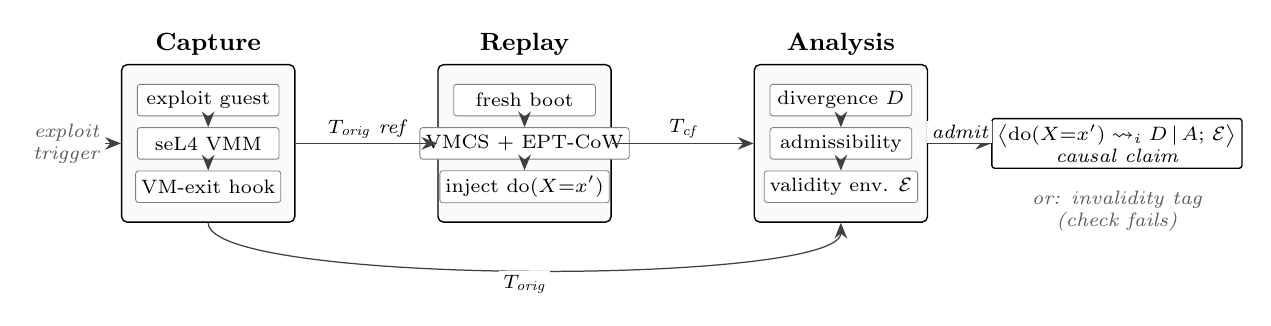
\begin{tikzpicture}[
    font=\footnotesize,
    >={Stealth[length=2mm,width=1.6mm]},
    every node/.style={inner sep=2pt},
    phase/.style={draw=black, line width=0.5pt, rounded corners=2pt,
                  minimum width=22mm, minimum height=20mm,
                  align=center, fill=black!2},
    sub/.style={draw=black!50, line width=0.3pt, rounded corners=1pt,
                font=\scriptsize, align=center,
                minimum width=18mm, minimum height=4mm, fill=white},
    flow/.style={->, line width=0.45pt, draw=black!75},
    tracelabel/.style={font=\scriptsize\itshape, fill=white, inner sep=1.5pt},
    diamond/.style={draw=black, line width=0.5pt,
                    diamond, aspect=1.6, align=center,
                    minimum width=14mm, minimum height=10mm,
                    font=\scriptsize, inner sep=1pt},
    output/.style={draw=black, line width=0.5pt, rounded corners=1pt,
                   align=center, font=\scriptsize,
                   minimum width=22mm, minimum height=6mm},
    notelabel/.style={font=\scriptsize\itshape, text=black!65}
  ]

  % ===== PHASE 1: CAPTURE =====
  \node[phase] (capture) {};
  \node[font=\small\bfseries] at (capture.north) [yshift=2.5mm] {Capture};
  \node[sub] (guest)   at ($(capture.center) + (0, 5.5mm)$) {exploit guest};
  \node[sub] (vmm1)    at ($(capture.center) + (0, 0mm)$)   {seL4 VMM};
  \node[sub] (vmexit)  at ($(capture.center) + (0,-5.5mm)$) {VM-exit hook};
  \draw[flow] (guest) -- (vmm1);
  \draw[flow] (vmm1)  -- (vmexit);

  % ===== PHASE 2: REPLAY =====
  \node[phase, right=18mm of capture] (replay) {};
  \node[font=\small\bfseries] at (replay.north) [yshift=2.5mm] {Replay};
  \node[sub] (boot)   at ($(replay.center) + (0, 5.5mm)$) {fresh boot};
  \node[sub] (restore)at ($(replay.center) + (0, 0mm)$)   {VMCS + EPT-CoW};
  \node[sub] (inject) at ($(replay.center) + (0,-5.5mm)$) {inject $\dox{x'}$};
  \draw[flow] (boot)    -- (restore);
  \draw[flow] (restore) -- (inject);

  % ===== PHASE 3: ANALYSIS =====
  \node[phase, right=18mm of replay] (analysis) {};
  \node[font=\small\bfseries] at (analysis.north) [yshift=2.5mm] {Analysis};
  \node[sub] (Dcheck)  at ($(analysis.center) + (0, 5.5mm)$) {divergence $D$};
  \node[sub] (admiss)  at ($(analysis.center) + (0, 0mm)$)   {admissibility};
  \node[sub] (envel)   at ($(analysis.center) + (0,-5.5mm)$) {validity env. $\mathcal{E}$};
  \draw[flow] (Dcheck) -- (admiss);
  \draw[flow] (admiss) -- (envel);

  % ===== INTER-PHASE FLOWS =====
  % T_orig: capture -> replay (as reference)
  \draw[flow] (capture.east) -- node[tracelabel,above]{$\Korig$ ref} (replay.west);

  % T_cf: replay -> analysis
  \draw[flow] (replay.east) -- node[tracelabel,above]{$\Tcf$} (analysis.west);

  % T_orig direct: capture -> analysis (curved, below)
  \draw[flow]
    (capture.south)
    .. controls +(0,-8mm) and +(0,-8mm) ..
    node[tracelabel,below,pos=0.5]{$\Korig$}
    (analysis.south);

  % ===== INPUT/OUTPUT =====
  % Input: exploit trace into capture
  \node[notelabel, left=2mm of capture.west, align=right]
    (input) {exploit\\trigger};
  \draw[flow] (input.east) -- (capture.west);

  % Output: emitted claim from analysis
  \node[output, right=8mm of analysis.east] (claim)
    {$\big\langle \dox{x'} \rightsquigarrow_i D \,|\, A;\,\mathcal{E}\big\rangle$ \\
     \scriptsize\itshape causal claim};
  \draw[flow] (analysis.east) --
    node[tracelabel,above,pos=0.5]{admit} (claim.west);

  % Alternative output (below): invalidity tag
  \node[notelabel, below=2mm of claim.south, align=center]
    {or: invalidity tag\\(check fails)};

  \end{tikzpicture}%
  }
  \caption{EXTp architecture. The exploit guest produces $\Korig$
    during capture (VM-exit observable surface plus per-event
    timing). $\Korig$ serves as the replay reference: in a fresh-boot
    session, the intervention $\dox{x'}$ is injected at the
    designated event's VM-entry boundary, producing $\Tcf$. Divergence
    detection $D$ fires on either 4-tuple difference (SOE clause) or
    timing excursion above $\Dstar$ (MI clause). If divergence is
    detected and the four-step CST admissibility check passes, EXTp
    emits a causal attribution claim.}
  \label{fig:arch}
\end{figure}

\subsection{Trace Capture and Fresh-Boot Replay}

EXTp's replay fidelity rests on two restore mechanisms operating in
concert. \emph{VMCS-level restore} resets 23 VMCS fields covering
guest control state, segment descriptors, and exception handling
(full enumeration in Appendix~\ref{app:vmcs}), plus RIP, RSP, RFLAGS,
and CR3, placing the virtual CPU in a clean initial state.
Non-restored fields are either constant across replay (host state)
or read-only (derived state).

\emph{EPT Copy-on-Write restore} reverts guest-modified physical
pages to their checkpoint state. The mechanism operates via EPT
permission downgrade: at checkpoint, all guest-writable pages are
marked read-only in the EPT; the first guest write to each page
triggers an EPT violation routed to
\texttt{extp\_ept\_cow\_handler()}, which allocates a shadow page,
copies the original content, and remaps the guest's view to the
shadow. Restore reverts each EPT mapping to the original page and
reclaims the shadow, returning the guest's memory view to its
pre-exploit state.

These two mechanisms handle the architectural state visible through
the VT-x interface. Microarchitectural state --- cache occupancy,
branch predictor history, TLB entries, MSR-resident state --- is not
reset by VMCS reload. EXTp addresses this through \emph{fresh-boot
discipline}: each counterfactual replay $\Tcf$ executes in an
independent boot session, not within the same boot as $\Korig$.
Cross-boot microarchitectural state is not preserved across power
cycles, providing a conservative reset guarantee. The cost is
measurement overhead; within-boot replay with explicit microarch
state reset machinery is future work.

Cross-boot replay's adequacy as a microarchitectural reset mechanism
is the empirical claim that SOE (\S\ref{sec:soe}) tests:
$\scoreS = 1.0000$ over $N{=}34$ cross-boot trials in the absence of
intervention is the operational evidence that fresh-boot discipline
produces deterministic 4-tuple trajectories.

\subsection{Intervention Machinery}\label{sec:intervention}

EXTp's intervention machinery modifies a designated parameter $X$ to
value $x'$ at a specified event $e_i$ during $\Tcf$'s execution.
Table~\ref{tab:interventions} summarizes the four validated
intervention classes.

\begin{table}[tb]
  \caption{EXTp intervention classes.}
  \label{tab:interventions}
  \centering
  \small
  \begin{tabular}{@{}p{0.13\textwidth}p{0.06\textwidth}p{0.08\textwidth}p{0.14\textwidth}@{}}
  \toprule
  Class & Type & Status & Mechanism \\
  \midrule
  nopcount       & Temp.\ & Validated   & Code patch, iter byte \\
  register write & State  & Implem.\    & \texttt{vcpu->regs} post-snap \\
  input value    & State  & Implem.\    & Hypercall arg rewrite \\
  cache preload  & State  & Future      & EPT + warmup pass \\
  \bottomrule
  \end{tabular}
\end{table}

The classification into \emph{state interventions} (input\_value,
reg\_state; cache\_state pending EPT warmup validation --- see
Table~\ref{tab:interventions}) and \emph{temporal interventions}
(nopcount) reflects the primary expected observable surface: state
interventions are designed to produce 4-tuple divergence; temporal
interventions are designed to produce timing divergence above
$\Dstar$. Both classes may trigger either clause of the divergence
detector $D$; the classification predicts, not constrains, the
expected signal.

Intervention scope in CST v1.0 is \emph{per-event}: $X$ is set to
$x'$ exactly at event $e_i$ and reverts thereafter; extended scopes
are discussed in \S\ref{sec:discussion}.

Compound interventions --- multiple modifications in the same $\Tcf$
--- are modeled as an ordered atomic sequence. Commutativity is not
assumed: $\text{do}(X_1{=}x_1') \rightarrow \text{do}(X_2{=}x_2')$
and $\text{do}(X_2{=}x_2') \rightarrow \text{do}(X_1{=}x_1')$ may
produce different divergence patterns if $X_1$'s effect alters the
state on which $X_2$ operates. Reordering analysis is a per-case
investigation, not a framework-level guarantee.

EXTp's admissibility check, detailed formally in
\S\ref{sec:cst}, takes the following operational form in the
framework: before issuing any causal claim, EXTp performs four
steps: (1)~the validity envelope $\mathcal{E}$'s tuple components
match CST v1.0 coverage; (2)~assumption validation references for
A1--A4 are present and current; (3)~divergence $D{=}\text{true}$ was
actually observed; (4)~$X$ is within the validated intervention
surface. Failure of any step produces a structured invalidity tag
rather than a claim (\S\ref{sec:cst}).

% =====================================================================
\section{Formal Properties}\label{sec:properties}

\subsection{Capability Separation (CapSep)}\label{sec:capsep}

\textbf{Proof structure.} CapSep is a hybrid structural-empirical
claim: structurally proven on $\Kverified$ by inheritance from
L4.verified, and empirically bounded on $\Kextended$ via
Clopper-Pearson confidence intervals on observed zero-failure trials.

\textbf{Claim.} $\Kint \cap \Kfwk = \emptyset$, where $\Kint$ is the
capability set held by EXTp's intervention machinery and $\Kfwk$ is
the capability set governing framework-internal state (VMM
scheduler, EPT structures outside the intervention surface,
capability registers not under intervention authority).

\textbf{Two-layer structure.} The disjointness claim has structurally
different strength on two operation classes introduced in
\S\ref{sec:background}:

For $\Kverified$ operations, disjointness follows from seL4's
L4.verified proof: the Isabelle/HOL functional correctness theorem
establishes external atomicity --- that every capability operation
in $\Kverified$ completes as an observable single step with no
intermediate state exposed. Because the intervention machinery's
authority set is a subset of $\Kextended$ and $\Kverified \cap
\Kextended = \emptyset$, authority disjointness on $\Kverified$ is
unconditional.

For $\Kextended$ operations (the VT-x extension API enumerated in
Appendix~\ref{app:kextended}), disjointness is empirically bounded.
Disjointness is tested by two complementary protocols, each
supporting a distinct downstream claim.

\textit{Within-boot} trials ($N{=}998$) measure authority leakage
within a single execution session and support \emph{comparator
reliability}: the protocol confirms that the intervention
machinery does not pollute its own observation surface when
running in steady state. Observed failure rate is zero;
Clopper-Pearson one-sided $95\%$ upper bound on the failure rate
is $\leq 0.37\%$.

\textit{Cross-boot} trials ($N{=}34$) measure authority leakage
across independent boot sessions and support \emph{A4's
operational bound}: the protocol confirms that residual
microarchitectural state from previous runs does not survive
fresh-boot discipline. Observed failure rate is zero;
Clopper-Pearson one-sided $95\%$ upper bound is $\leq 10.4\%$.
The wider cross-boot bound reflects the smaller sample (cross-boot
trials are operationally expensive). The within-boot bound is
the operational confidence value used in A1-modulo claims; the
cross-boot bound underwrites A4's replay-determinism antecedent
(\S\ref{sec:cst}).

\textbf{Pearl role.} Pearl's modularity axiom requires that
$\dox{x'}$ severs all incoming causal connections to $X$ in the
structural model. In EXTp's setting, ``incoming causal connections
to $X$'' correspond to capability-mediated authority over $X$'s
state. Disjointness $\Kint \cap \Kfwk = \emptyset$ therefore
establishes that intervention authority cannot reach $X$ via any
framework-internal pathway, satisfying modularity within the
capability-mediated subset of causal connections. The \emph{known
gap} below clarifies that non-capability side-effect paths (cache,
scheduler overhead) lie outside this subset.

\textbf{Known gap.} CapSep establishes \emph{authority disjointness},
not \emph{side-effect freedom}. The intervention machinery's
execution itself consumes microarchitectural resources --- VMM
scheduler time, cache lines, branch predictor history --- that may
produce indirect effects on framework state not governed by the
capability system. These side-effect paths are outside the
$\Kint \cap \Kfwk$ disjointness argument; their empirical
boundedness is the subject of the Q4 future experiment
(\S\ref{sec:discussion}). Until Q4 resolves, A1 (Pearl modularity;
formally stated in \S\ref{sec:cst}) in CST is asserted modulo
side-effects below $\Dstar$ on framework observables, and this
qualifier propagates: every CST claim's validity envelope
$\mathcal{E}$ carries an explicit \texttt{A1-modulo} flag; downstream
tools consuming CST claims must check this flag before relying on
causal attribution. All claims in this paper are issued under CST
v1.0 and carry this flag unless Q4 resolves otherwise.

\subsection{Strong Observational Equivalence (SOE)}\label{sec:soe}

\textbf{Proof structure.} SOE is a hybrid formal-empirical claim
with two antecedents: a structural antecedent (Capability
Separation, \S\ref{sec:capsep}) establishing that replay and original
execution operate under divergent authority, and an empirical
antecedent (comparator validity via four-field injection testing)
establishing that the 4-tuple comparator is faithful to its
specification.

\textbf{Claim.} Let $E$ be a guest execution under EXTp's VMM, and
$R = \text{replay}(E)$ the corresponding replay execution. Then:
\begin{equation}
E \approx_S R \quad \text{iff} \quad \forall i:\
\text{observable}(E)_i = \text{observable}(R)_i
\end{equation}
where the 4-tuple at event $i$ is
\begin{equation*}
\begin{aligned}
\text{observable}(X)_i = \langle\,&\text{rip}_i(X),\,\text{exit\_reason}_i(X), \\
                                  &\text{exit\_qual}_i(X),\,\text{rax}_i(X)\,\rangle.
\end{aligned}
\end{equation*}

\textbf{Empirical support.} Across $N{=}998$ single-boot replay
trials, $\scoreS = 1.0000$ (exact: zero failures on all four
observable fields across all events in all runs). Across $N{=}34$
cross-boot trials, $\scoreS = 1.0000$ again. Clopper-Pearson
one-sided $95\%$ upper confidence bounds on the per-run failure rate
are $\leq 0.37\%$ at $N{=}998$ and $\leq 10.4\%$ at $N{=}34$. The
$N{=}34$ cross-boot bound is the conservative public-facing figure
cited in the introduction; the tighter $N{=}998$ bound is the
operational value. In either case, the ``$1.0000$'' framing is
\emph{high-confidence empirical}, not categorical.

\textbf{Scope limitation.} The observable surface covers RAX as the
sole general-purpose register. Other GPRs (RBX, RCX, RDX, R8--R15)
are captured internally but excluded from the formal surface for
falsifiability: a surface defined over all 16 GPRs would require
determinism claims over register state that EXTp's current
calibration does not support. Exploits whose divergence manifests
exclusively in non-RAX registers are silent on the SOE surface ---
a scope boundary analogous to MI's silent-leak class. Extension to
the full register file is straightforward mechanically but requires
$N$-trial recalibration; deferred (\S\ref{sec:discussion}).

\textbf{Pearl role.} SOE underwrites two assumptions: A4 (replay
determinism) and, through its 4-tuple surface definition, A2
(observable surface coverage) --- both formally stated in
\S\ref{sec:cst}. SOE's trajectory-level reproducibility is
\emph{strictly stronger} than Pearl's probabilistic faithfulness
axiom: faithfulness requires that conditional independences in an
observed distribution correspond to d-separations in the underlying
DAG, which presupposes a probability distribution. Under SOE's
deterministic replay, there is no distribution --- trajectories are
reproduced exactly, making probabilistic CI testing unnecessary. A4
therefore inherits a property stronger than faithfulness requires,
which is why CST's proof sketch (\S\ref{sec:cst}) does not appeal to
CI testing at any step.

\subsection{Measurement Interference (MI)}\label{sec:mi}

\textbf{Proof structure.} MI is an empirical claim grounded in two
antecedents: (i)~$\sigbase$ estimation from post-warmup
zero-perturbation samples per workload class and instrument, and
(ii)~FPR validation against nominal $\alpha$ via Clopper-Pearson
confidence intervals on observed false-positive counts.

\textbf{Claim.} For workload class $L$ under timing instrument $S$,
there exists a calibrated detection threshold $\Dstar = z_{1-\alpha}
\cdot \sigbase$ such that a per-event timing deviation above
$\Dstar$ is detectable with false-positive rate bounded by $\alpha$
(nominal $0.05$). $\sigbase$ is the sample standard deviation of
post-warmup timing samples at zero perturbation ($\text{iter}{=}0$),
computed within each experiment.

\textbf{Timing instruments.} EXTp supports two instruments. $S_1$
(LFENCE-sandwich-RDTSC) serializes instruction retirement before the
TSC read, adding ${\sim}3\times$ noise over $S_2$ (bare RDTSC) but
eliminating out-of-order TSC read artifacts. $S_2$ is preferred for
detection-threshold calibration; $S_1$ for cross-workload
comparisons requiring serialization consistency.

\textbf{Calibrated values.} For the $L_1$-pchase workload class
under $S_1$: $\sigbase = 5{,}518$ cycle ($n{=}108$,
boot\_log12, iter$=0$), slope $b = 4.481$ cycle/iter, $\Dstar =
1.645 \times 5{,}518 = 9{,}077$ cycle. For $L_2$-pchase under $S_2$
(boot\_log15, $n{=}108$, iter$=0$): $\sigbase = 4{,}604$ cycle,
$b = 15.194$ cycle/iter, $\Dstar = 1.645 \times 4{,}604 = 7{,}574$
cycle. The $\hat{\sigma}$ confidence interval at $n{=}108$ is
$[4{,}867,\, 6{,}371]$ cycle ($95\%$), implying a $\Dstar$
uncertainty range of approximately $+15\%/{-}12\%$ (asymmetric,
reflecting the $\chi^2$ CI structure on $\hat{\sigma}$; upper:
$1.645 \times 6{,}371 = 10{,}480$ cycle; lower: $1.645 \times 4{,}867
= 8{,}006$ cycle). This is $\hat{\sigma}$-noise dominated, not a
functional-form mismatch (\S\ref{sec:eval}).

\textbf{Empirical FPR.} Realized false-positive rate is
workload-dependent. For $L_1$-pchase under $S_1$ (boot\_log8,
$n{=}978$): $0.61\%$ (Clopper-Pearson $95\%$ CI
$[0.22\%, 1.33\%]$). For $L_1$-pchase under $S_1$ at finer grain
(boot\_log12, iter$=0$, $n{=}108$): $2.78\%$ (CI
$[0.58\%, 7.91\%]$). Both lie below nominal $\alpha{=}5\%$; the
wider boot\_log12 interval reflects the smaller $n$.

The use of $z = 1.645$ (Gaussian one-sided $\alpha{=}5\%$
quantile) for $\Dstar$ calibration is a deliberate design choice,
not a distributional assumption: when the empirical timing
distribution has heavier-than-Gaussian tails (as observed under
$L_1$-pchase, where the empirical-to-nominal FPR ratio is
${\approx}8.2{\times}$ for boot\_log8), the Gaussian threshold
over-estimates tail probability and therefore yields empirical
FPR strictly below the nominal $\alpha$. This is conservative in
the false-positive direction by construction. The cost is reduced
detection sensitivity for effects near $\Dstar$; this trade-off
is intentional and is consistent with EXTp's broader emphasis on
sound (rather than complete) attribution.

\textbf{Scope: per-event detection.} MI claims per-event
detection-threshold validity. The detection criterion's $\alpha$ is
per-event: each event-indexed comparison carries nominal
false-positive rate $\alpha$. For a trace of $N$ events, the
expected false detection count under no perturbation is
$N \cdot \arealized$. Trace-level false discovery rate (FWER) is the
downstream consumer's aggregation responsibility; MI does not
prescribe a correction method, as the appropriate correction depends
on the consumer's use case.

\textbf{Pearl role.} MI underwrites A3 (formally stated in
\S\ref{sec:cst}): timing deviations above $\Dstar$ are attributable
to intervention rather than baseline noise, at the calibrated FPR.
A3 is an EXTp-specific assumption addressing the empirical noise
floor absent from Pearl's idealized structural equations; it
captures confounder boundedness in the timing domain and complements
Pearl's axioms rather than mapping directly to any one of them.
MI's $\Dstar$ extends SOE's 4-tuple surface (A2, \S\ref{sec:cst})
into the timing domain, enabling detection of interventions whose
causal effect is temporal rather than structural.

\subsection{Counterfactual Soundness Theorem (CST)}\label{sec:cst}

\textbf{Proof structure.} CST is the binding theorem of the property
hierarchy: it formally proves that the three observable properties
(CapSep, SOE, MI) compose into sound causal attribution. CST does
not make new empirical claims; it asserts that CapSep + SOE + MI, in
composition, are sufficient to ground Pearl-style causal attribution
within enumerated epistemic bounds.

\begin{theorem}[CST Composition Closure, atomic case]
\label{thm:cst}
Let $\Korig$ and $\Tcf$ be counterfactual replays under a single
configuration, with $\Tcf$ generated by atomic intervention
$\dox{x'}$. Let $A = (A_1, A_2, A_3, A_4)$ be the assumption envelope
and $\mathcal{E}$ the validity envelope. Under $A$ satisfied and
$\mathcal{E}$ admitted, the atomic CST claim
$$\big\langle \dox{x'} \rightsquigarrow_i D \;\big|\;
A;\;\mathcal{E} \big\rangle$$
is \emph{admissible} iff $D(\Korig, \Tcf, i) = \text{true}$ and the
four-step admissibility check (\S\ref{sec:intervention}) passes.
When admissible, the claim asserts that observable divergence $D$ at
event $i$ is causally attributable to $\dox{x'}$, without making
claims about the microarchitectural mechanism by which the
divergence arose. Furthermore, the admissible claim satisfies:
\begin{enumerate}[label=(\roman*)]
\item Pearl's effectiveness axiom: $\dox{x'}$ sets $X$ to $x'$;
\item Pearl's composition axiom in a $\delta_{\text{A1}}$-relaxed
  form: composition holds with $W_\text{cf} - W_\text{orig}$
  bounded by $\delta_{\text{A1}}$ (CapSep \S\ref{sec:capsep}) rather
  than exactly equal. The strict Pearl form is recovered in the
  $\delta_{\text{A1}} \to 0$ limit; CST v1.0 operates with
  $\delta_{\text{A1}} \leq 0.37\%$ (within-boot) /
  $\leq 10.4\%$ (cross-boot). The Q4 modularity experiment
  (\S\ref{sec:discussion}) targets strict-form recovery by
  validating side-effect freedom directly;
\item Halpern-Pearl AC1: effect $D$ occurs in the counterfactual
  trace $\Tcf$;\footnote{AC1's ``actual world'' in CST is $\Tcf$ ---
  the world in which the intervention was applied and the divergence
  observed. This differs from the classical HP framing where the
  actual world is pre-intervention.}
\item Halpern-Pearl AC2(a): effect $D$ differs from $\Korig$ under
  intervention, establishing counterfactual sensitivity. AC2(b)
  [witness fixity]: we construct the HP witness set
  $W = \mathcal{S}_\text{in} \setminus \{\text{observable}(\cdot)_i\}$
  from the validity envelope's $\mathcal{S}_\text{in}$ specification
  and verify the two HP witness conditions --- (W1) fixity
  enforceability discharged by A4, and (W2) the
  fixity-does-not-mask condition discharged jointly by
  Lemma~\ref{lem:coincidence-soe} and
  Lemma~\ref{lem:confounder}. The witness-fixity construction is
  derived in full in Appendix~\ref{app:proofs}, Composition into
  Theorem~\ref{thm:cst}, item~(iv), which also refines the residual
  envelope per witness clause (structural vs.\ timing), with which
  is tighter depending on the calibration regime.
\end{enumerate}
\end{theorem}

\textbf{Assumptions.} Table~\ref{tab:assumptions} states the four
assumptions formally. Each derives from an upstream property entry.

\begin{table}[tb]
  \caption{CST assumptions.}
  \label{tab:assumptions}
  \centering
  \small
  \begin{tabular}{@{}p{0.11\textwidth}p{0.13\textwidth}p{0.06\textwidth}p{0.10\textwidth}@{}}
  \toprule
  Assump.\ & Role & Source & Status \\
  \midrule
  A1 Modul.\           & $\text{do}()$ side-eff.\ free & CapSep
                       & Mod.\ Q4 \\
  A2 Obs.\ comp.\      & Scope-compl.\                 & SOE
                       & Mod.\ silent \\
  A3 Confound.\        & Noise $<\Dstar$               & MI
                       & Calibrated \\
  A4 Determ.\          & No coincidence                & SOE
                       & High-conf. \\
  \bottomrule
  \end{tabular}

  \vspace{0.3em}
  \footnotesize{Source columns: CapSep~(\S\ref{sec:capsep}),
  SOE~(\S\ref{sec:soe}), MI~(\S\ref{sec:mi}). A2 silent-channel
  qualifier per~\S\ref{sec:threat}. A4 confidence $N{=}34$.}
\end{table}

\textbf{Proof argument structure: threat elimination.} We adopt a
threat-elimination structure (rather than direct
antecedent$\rightarrow$conclusion derivation) because the three
threats correspond directly to the empirical gaps motivating EXTp's
three properties; a rigorous formal derivation following standard
proof structure is in Appendix~\ref{app:proofs}. The proof addresses
three threats in turn.

\emph{Threat 1 --- Coincidence.} Under A4 (replay determinism,
grounded by SOE's $\scoreS = 1.0000$ over $N{=}34$ cross-boot
trials), spontaneous divergence on the 4-tuple surface is ruled out
at false-positive rate zero: any 4-tuple divergence in $\Tcf$
relative to $\Korig$ requires a trace-distinguishing input
difference; under the single-configuration discipline, the only
controlled trace-distinguishing input is $\dox{x'}$. External
factors (microcode jitter, thermal variance, hardware faults) are
bounded by SOE's empirical $\scoreS = 1.0000$ over $N{=}34$
cross-boot trials; attribution to $\dox{x'}$ is the
maximum-likelihood explanation within the calibrated confidence
envelope. The timing clause admits a residual coincidence rate
$\arealized$, calibrated per workload class ($0.61\%$ under
$L_1$-pchase/$S_1$ boot\_log8; $2.78\%$ under $L_1$-pchase/$S_1$
boot\_log12; MI \S\ref{sec:mi}), incorporated into A3 as an
explicitly bounded, not silenced, source of attribution uncertainty.

\emph{Threat 2 --- Silent mechanism.} Addressed by scope-honesty
under A2. If a silent microarchitectural process triggered by
$\dox{x'}$ produces no 4-tuple delta and no timing deviation above
$\Dstar$, then $D = \text{false}$ and CST issues no claim ---
scope-honest silence. If the silent process does produce observable
divergence, $D = \text{true}$ and CST attributes correctly at the
event-chain level, mechanism-agnostic: CST claims that $\dox{x'}$
caused the observable divergence, not that it caused the underlying
microarchitectural change. Silent processes that manifest neither
clause of $D$ are explicitly deferred to a future CMD
property class (\S\ref{sec:discussion}).

\emph{Threat 3 --- Confounder.} Addressed by A1 (modularity,
grounded by CapSep \S\ref{sec:capsep}), modulo the known gap. Under
A1, intervention execution does not modify framework-internal state
outside $X$'s capability authority scope; no third factor correlated
with $\dox{x'}$ can produce the divergence. Until the side-effect
quantification experiment resolves (Q4; \S\ref{sec:discussion}), A1
is asserted modulo side-effects below $\Dstar$: framework-internal
side-effects bounded below the detection threshold are absorbed into
A3's noise model rather than constituting unbound confounders
(propagated per-claim via the \texttt{A1-modulo} flag,
\S\ref{sec:capsep}).

\textbf{Compositional extension.}
\begin{proposition}[Sequential composition]
$\langle \text{do}(X_1) \rightsquigarrow_{i_1} \cdots
\rightsquigarrow_{i_n} D \mid A; \mathcal{E}\rangle$ is admissible
iff every atomic step is independently admissible under
Theorem~\ref{thm:cst}.
\end{proposition}

\emph{Proof sketch by induction on chain length:} the base case is
Theorem~\ref{thm:cst}; the inductive step requires that A1's
framework-state isolation propagates across sequential interventions,
which follows from CapSep's per-operation disjointness --- each
$\Kint$ operation remains disjoint from $\Kfwk$ regardless of
execution order. Commutativity is not assumed. Full proof in
Appendix~\ref{app:proofs}.

\textbf{Pearl/HP correspondence.}
Table~\ref{tab:pearl} summarizes CST's correspondence to Pearl's
structural causal model and Halpern-Pearl actual-causation
conditions.

\begin{table}[tb]
  \caption{Pearl/HP correspondence with explicit deviation modes.}
  \label{tab:pearl}
  \centering
  \footnotesize
  \begin{tabular}{@{}p{0.085\textwidth}p{0.13\textwidth}p{0.075\textwidth}p{0.08\textwidth}@{}}
  \toprule
  Construct & EXTp realization & Status & Relationship \\
  \midrule
  Modularity      & CapSep: $\Kint \cap \Kfwk = \emptyset$ & Holds mod A1     & Relaxed-$\delta_{\text{A1}}$ \\
  Effectiveness   & Intervention (\S\ref{sec:intervention})       & Holds            & Direct \\
  Composition     & Inherits A1 modularity         & Holds mod A1     & Relaxed-$\delta_{\text{A1}}$ \\
  Reversibility   & Linear-time exec.              & Inapplicable     & Inapplicable \\
  do-calc. R1--3  & Degenerate-determ.             & Hold             & Stronger \\
  Faithfulness    & Subsumed by A4 (SOE)           & Subsumed         & Stronger \\
  HP AC1          & $D$ in $\Tcf$ at $i$           & Direct           & Direct \\
  HP AC2(a)       & $D$ differs in $\Korig$        & Direct           & Direct \\
  HP AC2(b)       & Witness fix.\ via fresh-boot   & Direct (App.~\ref{app:proofs}) & Direct \\
  HP AC3 (min.)   & Future work                    & Out of scope     & Deferred \\
  \bottomrule
  \end{tabular}
\end{table}

The \emph{Relationship} column in Table~\ref{tab:pearl} makes
explicit the four distinct ways in which CST's apparatus relates
to Pearl's classical framework. \emph{Direct} entries hold as
straightforward correspondences without modification
(effectiveness; HP AC1, AC2(a), AC2(b)). \emph{Stronger} entries
are properties that EXTp's deterministic setting satisfies in a
form strictly stronger than Pearl's probabilistic original ---
faithfulness is subsumed by SOE's trajectory-level determinism
(\S\ref{sec:soe}), and do-calculus rules R1--R3 reduce to
trajectory equality testing under A4. \emph{Relaxed-$\delta_{\text{A1}}$}
entries are properties that hold in an approximate form bounded by
CapSep's empirical envelope (\S\ref{sec:capsep}): modularity and
composition are established to within $\delta_{\text{A1}}$ rather
than exactly, with the strict Pearl form recovered in the
$\delta_{\text{A1}} \to 0$ limit (which Q4 future work targets,
\S\ref{sec:discussion}). \emph{Inapplicable} entries are Pearl
constructs whose preconditions do not arise in EXTp's setting ---
reversibility requires algebraic intervention reversal within a
single structural model, which has no analog under linear-time
bare-metal execution. We declare these four modes explicitly
rather than collapsing them under a single ``holds modulo''
qualifier; downstream consumers of CST claims can therefore
distinguish strengthening from relaxation when assessing claim
transportability.

AC3 (minimality over the cause set) is outside CST v1.0 scope: CST
issues \emph{causal-link} claims --- attributing observable
divergence to a named intervention --- not
\emph{causal-explanation} claims identifying the minimal sufficient
cause set. Extension to AC3 requires a search procedure over
candidate intervention sets and is deferred.

% =====================================================================
\section{Evaluation}\label{sec:eval}

\subsection{Experimental Setup}

All experiments run on bare-metal Intel 12th Gen Core (Alder Lake,
microcode \texttt{0x3e}, ASUS Z690 motherboard, UEFI firmware) with
no host OS. The seL4 VMM runs directly on hardware; the guest
executes under EXTp's VT-x control loop. Serial console infrastructure
(DIGITUS USB-Serial FT232RL, Digitus PCIe Serial DS-30000-1, RS-232
null modem cable) provides out-of-band I/O during bare-metal runs.
No network connectivity is present during any experiment.

All timing measurements use bare RDTSC ($S_2$) for
detection-threshold calibration and LFENCE-sandwich-RDTSC ($S_1$)
for cross-workload comparisons. EXTp's VMM is compiled with gcc 12.3
at \texttt{-O2} (build hash in Appendix~\ref{app:build}).

\subsection{Privilege-Check-Bypass Demonstration}\label{sec:eval-demo}

The demonstration exercises EXTp's full attribution pipeline on a
synthetic capability-bypass exploit pattern modeled on the
CrackArmor confused-deputy class (\S\ref{sec:intro}, C4).
\emph{A synthetic analog is used rather than a real CrackArmor
instance for a soundness-preserving reason, not a convenience one:}
real CrackArmor exploits exercise multi-VCPU code paths (concurrent
privilege-check races between cooperating threads) that lie outside
CST v1.0's single-VCPU envelope (\S\ref{sec:threat}, Out of Scope
item~1). Running EXTp against a real CrackArmor trace would produce
admissibility-check failures at step~(1) --- envelope mismatch ---
and would not yield a CST claim under any intervention, by design.
The synthetic analog isolates the structural pattern CrackArmor
exploits (capability-token forgery producing privileged-path
divergence) within the single-VCPU regime where A4's replay
determinism holds, allowing the full attribution pipeline to
execute end-to-end.

The scenario preserves the confused-deputy causal structure of the
original CVE class --- a token-mediated privilege check that, when
bypassed, branches execution into a privileged path --- while
maintaining the single-VCPU determinism CST v1.0 requires. It
produces both a clean SOE-clause divergence signal at event~1 and
an empirical surface on which the timing clause and the A1-modulo
bound can be independently observed
(\S\ref{sec:eval-demo}, subsequent subsubsections).

\subsubsection{Scenario}

A 29-byte synthetic guest binary at GPA \texttt{0x10000} executes a
control flow that branches on a capability token held in register
\texttt{r8}.\footnote{\texttt{r8} is used rather than \texttt{rax}
because the VMM's CPUID handler deterministically writes the
``EXTp'' vendor ID into \texttt{rax}--\texttt{rdx} on every CPUID
exit (\S\ref{sec:framework}), clobbering those registers; \texttt{r8}
is preserved across CPUID handling, making it a faithful carrier of
the capability-token state across event boundaries.} The default
path (\texttt{r8 = 0}) executes a benign CPUID at offset 13
(RIP \texttt{0x1000d}, RAX cleared); the privileged path
(\texttt{r8 = 0xDEAD}) executes CPUID at offset 22
(RIP \texttt{0x10016}, RAX \texttt{0x80000008}).
Table~\ref{tab:demo-divergence} shows the predicted and observed
divergence at event 1.

\begin{table}[tb]
  \caption{Demo divergence prediction (matches observation across
    all $N{=}200$ post-warmup trials, bare-metal Intel Alder Lake
    per \S\ref{sec:eval}).}
  \label{tab:demo-divergence}
  \centering
  \small
  \begin{tabular}{@{}cp{0.13\textwidth}p{0.14\textwidth}@{}}
  \toprule
  Event & $\Korig$ (\texttt{r8=0}) & $\Tcf$ (\texttt{r8=0xDEAD}) \\
  \midrule
  0 & RIP \texttt{0x10000}, CPUID, RAX 0    & identical \\
  1 & RIP \texttt{0x1000d}, CPUID, RAX 0    & RIP \texttt{0x10016}, CPUID, RAX \texttt{0x80000008} \\
  2 & RIP \texttt{0x10018}, VMCALL          & identical \\
  \bottomrule
  \end{tabular}
\end{table}

The intervention $\text{do}(\text{r8}{=}\text{0xDEAD})$ fires
immediately after the CPUID handler completes for event~0, via a
second \texttt{WriteRegisters} call that overrides \texttt{r8} while
preserving all other registers from the handler's state. The guest
then executes \texttt{cmp \$0xDEAD, \%r8} at offset~2 with the
forged token, takes the conditional branch, and follows the
privileged path through event~1's CPUID. Event~2's VMCALL terminates
both traces identically (post-divergence reconvergence).

\subsubsection{SOE-clause divergence}

Across $N{=}100$ same-condition pairs and $N{=}100$ cross-condition
pairs (single-boot run, 222 total runs minus 22 framework- and
inner-warmup-discarded samples), the four-step admissibility check
(\S\ref{sec:intervention}) passes for every trial:
\begin{enumerate}[label=(\arabic*)]
\item Envelope match: instrument $S_1$, workload class
  \textit{synthetic-guest}, intervention scope per-event at event~0,
  hardware identity Alder Lake / microcode \texttt{0x3e} / Z690.
\item Assumption validation: A1--A4 references current; A1 carries
  the \texttt{A1-modulo} flag (\S\ref{sec:capsep}).
\item Surface check: $D(\Korig, \Tcf, 1) = \text{true}$ via the SOE
  clause --- RIP and RAX both diverge.
\item Intervention surface: \texttt{r8} $\in$ \texttt{\{reg\_state\}}
  intervention class.
\end{enumerate}
The admissible CST claim emitted in every trial is:
\begin{equation*}
\big\langle \text{do}(\text{r8}{=}\text{0xDEAD}) \rightsquigarrow_{1}
D \,\big|\, A_1^{\text{mod}}, A_2, A_3, A_4;\, \mathcal{E}_{\text{v1.0}} \big\rangle
\end{equation*}
The SOE clause fires with false-positive rate zero (deterministic
4-tuple equality under A4's $\scoreS{=}1.0000$ guarantee): the RIP
delta $\text{0x1000d} \to \text{0x10016}$ and RAX delta
$\text{0x0} \to \text{0x80000008}$ are observed in every
cross-condition pair, and zero divergences are observed in any
same-condition pair.

\subsubsection{Timing-clause behavior and the A1-modulo bound}

The same demonstration was run under two implementations of the
intervention machinery, exposing the timing clause's sensitivity to
the A1-modulo gap (\S\ref{sec:capsep}).

\paragraph{Silent hook (production).} The deployed implementation
gates all informational output from the intervention apparatus
(error paths excepted). Across $N{=}100$ per condition, the
synthetic workload's baseline timing standard deviation is
$\sigbase = 6{,}237$ cycle (Clopper-Pearson via $\chi^2$ CI:
$[5{,}476,\, 7{,}245]$, half-width $-12.2\%/+16.2\%$). The realized
threshold is $\Dstar = 1.645 \cdot 6{,}237 = 10{,}259$ cycle. The
intervention signature is
\begin{equation*}
\overline{T_\text{cf}} - \overline{T_\text{orig}} = +342 \text{ cycle} \approx 0.03 \cdot \Dstar
\end{equation*}
(${\approx}70$~ns at 4.9~GHz; one extra \texttt{WriteRegisters}
syscall accounts for this magnitude). The timing clause of $D$ is
\textbf{subthreshold} in every trial: the SOE clause is the sole
divergence signal, and the A1-modulo bound holds at paper-grade
$N$. Figure~\ref{fig:demo-silent} shows the timing distribution.

\paragraph{Naïve hook (counter-demonstration).} An earlier
implementation of the same intervention included an informational
\texttt{printf} in the hook's success path. Under this
implementation, at $n{=}23$ per condition, the intervention
signature is
\begin{equation*}
\overline{T_\text{cf}} - \overline{T_\text{orig}} = +26{,}617{,}599 \text{ cycle} \approx 2{,}595 \cdot \Dstar
\end{equation*}
where $\Dstar = 10{,}259$ cycle is the authoritative threshold
calibrated under the silent-hook implementation
(\S\ref{sec:eval-demo} above; the naïve-hook trace's own sample
standard deviation $7{,}727$ cycle reflects an A1-modulo-broken
state contaminated by printf I/O latency and is not used as a
detection threshold). The magnitude
$26.6$M cycle $\approx 5.43$~ms at 4.9~GHz is itself
diagnostically informative: at 115200-baud synchronous serial
output, $\sim$60 characters of \texttt{printf} yield $\sim$5~ms
of I/O latency, matching the observed signature. The SOE clause
fires identically in both implementations (the 4-tuple delta is
determined by the guest's branch target, not by hook latency),
but the timing clause fires for the \emph{wrong reason} under the
naïve hook: not because the guest's causal effect is detectable
on the timing surface, but because the intervention apparatus's
own execution cost exceeds $\Dstar$ by three orders of magnitude.
Figure~\ref{fig:demo-comparison} shows the contrast.

\begin{figure}[tb]
  \centering
  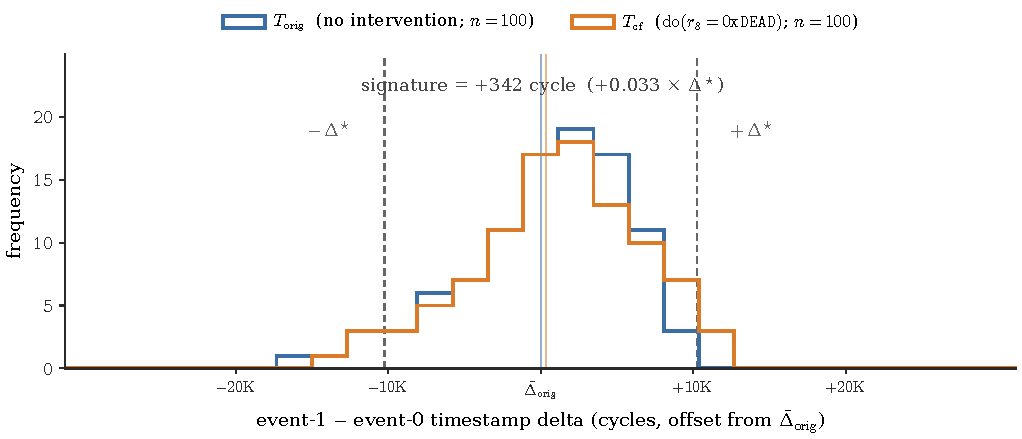
\includegraphics[width=0.95\columnwidth]{fig/paper_section6_silent_histogram.pdf}
  \caption{Silent-hook demonstration: timing distribution of
    $\Korig$ vs $\Tcf$ ($N{=}100$ per condition). The intervention
    signature ($+342$ cycle, $0.03\cdot\Dstar$) is dwarfed by the
    detection threshold (dashed red, $\pm\Dstar = \pm10{,}259$
    cycle). Distributions overlap heavily, consistent with
    A1-modulo holding under the silent implementation.}
  \label{fig:demo-silent}
\end{figure}

\begin{figure}[tb]
  \centering
  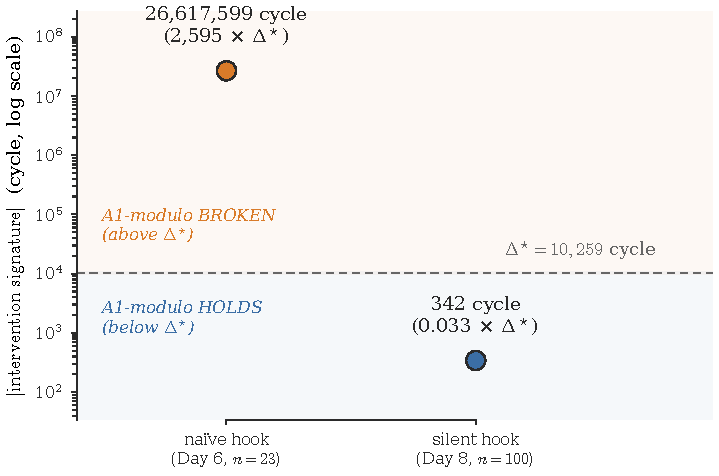
\includegraphics[width=0.95\columnwidth]{fig/paper_section6_signature_comparison.pdf}
  \caption{Intervention signature magnitude under two hook
    implementations, compared against the authoritative detection
    threshold $\Dstar = 10{,}259$ cycle (silent-hook calibration,
    dashed). The naïve hook ($n{=}23$, Day 6): signature
    $+26{,}617{,}599$ cycle $\approx 2{,}595\cdot\Dstar$, A1-modulo
    \emph{broken} (printf I/O latency dominates the timing surface).
    The silent hook ($n{=}100$, Day 8): signature $+342$ cycle
    $\approx 0.033\cdot\Dstar$, A1-modulo \emph{holds} (intervention's
    own execution cost is well below the detection threshold). The
    SOE-clause divergence is identical in both implementations; only
    the timing clause distinguishes them.}
  \label{fig:demo-comparison}
\end{figure}

\subsubsection{Reading: the framework detects its own A1 violations}

This bifurcation is, on its face, a story about instrumentation
discipline: silent hooks pass the A1-modulo check; verbose hooks do
not. But the structural point for CST is sharper. The naïve-hook
data is not a bug-fix anecdote; it is an \emph{operational test} of
CST's own assumption envelope. The naïve hook produces an
intervention apparatus whose execution cost on the timing surface
($+26.6$M cycle) demonstrably exceeds $\Dstar$ --- precisely the
condition under which A1's modulo qualifier fails. The framework's
timing clause correctly fires; CST's admissibility check correctly
attaches the \texttt{A1-modulo} flag; downstream consumers reading
that flag are correctly warned that the timing surface contains a
machinery contribution. The silent hook restores A1-modulo and
returns the timing clause to its design-intended role
(intervention-effect detection rather than machinery-cost detection).
The SOE clause is invariant across both implementations because
4-tuple determinism is a property of the guest's causal structure,
not the hook's instrumentation overhead --- the structural feature
that makes SOE the robust attribution signal under A4.

\subsubsection{Counterfactual sweep: causal coverage map}
\label{sec:eval-demo-sweep}

The single-intervention demonstration above establishes that
$\dox{r_8{=}\text{0xDEAD}}$ produces an admissible CST claim. To
test whether the same admissibility machinery correctly handles
the broader fuzzing-style sweep CST is designed to support
(\S\ref{sec:discussion-fuzz}), we ran a 33-value sweep over $r_8$
$\in S_{r_8}$ on the same bare-metal configuration, where
$S_{r_8}$ contains the validated exploit value
(\texttt{0xDEAD}), 16 low-byte values (\texttt{0x0}--\texttt{0xF})
spanning the structural-collision region, 14 wide-pattern values
(\texttt{0x1111}, \texttt{0x2222}, $\ldots$, \texttt{0xEEEE}),
and the two semantic distractors \texttt{0xCAFE} and
\texttt{0xBEEF}. Each of the 33 $r_8$ values is applied as an
\emph{independent atomic intervention} at event~0; the sweep is a
\emph{parallel ensemble} of Theorem~\ref{thm:cst} instances rather
than a sequential composition under Proposition~1. Each run begins
from an independent fresh-boot state, applies a single
$\text{do}(r_8{=}v)$ at the designated event, and is evaluated
against $\Korig$ by the same atomic admissibility check
(\S\ref{sec:intervention}). The $\delta_{\text{A1}}$ modulo bound
therefore applies per-instance and does not accumulate across the
sweep. Each value was applied twice (66 $\Tcf$ runs total) under
the silent-hook implementation.

\textbf{Result.} The divergence count is $1/33$, matching the
binary scenario design exactly: only $r_8 = \text{0xDEAD}$
triggered the privileged path (RIP $0x10016$, RAX
\texttt{0x80000008}, SOE clause firing); all 32 other values
followed the default path (RIP $0x1000d$, RAX 0, SOE clause
silent). Within-input reproducibility was $100\%$: every $r_8$
value produced an identical event-1 4-tuple across both of its
repeat passes, extending A4's determinism guarantee from the
no-intervention baseline ($\scoreS{=}1.0000$ over $N{=}34$
cross-boot, \S\ref{sec:soe}) to the intervention-applied case
across the full sweep. Figure~\ref{fig:demo-sweep} visualizes the
verdict map.

This map instantiates the witness-refined ensemble envelope of
Appendix~\ref{app:proofs}: one admissible claim (structural clause)
among 32 scope-honestly silent inputs that emit no claim, so the
sweep's aggregate envelope is that of a single structural claim
($1.35\%$ within-boot), not the $33{\times}$ figure a per-input
accounting would suggest. The instantiation is machine-checked
(\S\ref{sec:discussion-isabelle}).

\begin{figure}[tb]
  \centering
  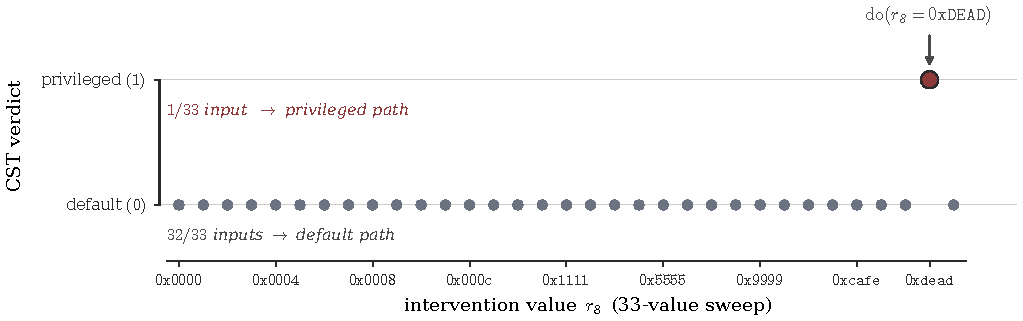
\includegraphics[width=0.95\columnwidth]{fig/paper_section6_fuzz_causal_map.pdf}
  \caption{Counterfactual fuzzing causal map. CST verdict for
    each of the 33 swept $r_8$ values: 32 default-path inputs
    (gray, $D{=}\text{false}$, SOE clause silent, no admissible
    divergence claim) versus the single privileged-path input
    \texttt{0xDEAD} (dark red, $D{=}\text{true}$, SOE clause
    fires, admissible CST claim emitted). The envelope over this
    exact 32/1 sweep is machine-checked
    (\texttt{dead\_sweep\_envelope\_vs\_naive\_swept},
    Table~\ref{tab:mechanized}). The 33-input sweep
    demonstrates the falsifiability primitive: the framework's
    verdict separates structurally on $D$'s observable predicate,
    rather than on heuristic crash signatures or aggregate metrics.
    This is mechanism evidence, not a fuzzing benchmark; sweep
    coverage and discovery-rate evaluation are out of scope for
    CST v1.0.}
  \label{fig:demo-sweep}
\end{figure}

\textbf{Reading.} The sweep is the operational instance of what
CST-grounded fuzzing produces: a per-input causal coverage map
where each point is labeled by admissibility verdict rather than
crash signature. Two structurally distinct failure modes (silent
admissibility with $D{=}\text{false}$ versus admissible
divergence with $D{=}\text{true}$) are reported as distinct
output classes by the same framework, with no heuristic
acceptance threshold introduced between them. The
single-shot $n{=}2$-per-value confidence is mechanically modest;
the structural claim is that admissibility is a falsifiable
classifier, separately verifiable per input. The downstream
implications for counterfactual fuzzing are discussed in
\S\ref{sec:discussion-fuzz}.

\subsection{Measurement Characterization}\label{sec:eval-meas}

Table~\ref{tab:meas} reports $\sigbase$, $\Dstar$, realized FPR, and
$\scoreS$ across the three workload classes characterized to date:
the two pchase reference workloads from MI calibration
(\S\ref{sec:mi}) and the synthetic-guest workload introduced by the
demonstration (\S\ref{sec:eval-demo}).

\begin{table}[tb]
  \caption{Measurement characterization.}
  \label{tab:meas}
  \centering
  \small
  \begin{tabular}{@{}llrrrr@{}}
  \toprule
  Workload      & Instr & $\hat{\sigma}$ & $\Dstar$    & FPR     & $\scoreS$ \\
  \midrule
  $L_1$-pchase  & $S_1$ & $5{,}518$      & $9{,}077$   & $0.61\%$ & $1.0000$ \\
  $L_2$-pchase  & $S_2$ & $4{,}604$      & $7{,}574$   & $2.78\%$ & $1.0000$ \\
  Synth.\ guest & $S_1$ & $6{,}237$      & $10{,}259$  & subthresh.\ & $1.0000$ \\
  \bottomrule
  \end{tabular}

  \vspace{0.3em}
  \footnotesize{Pchase rows: $N{=}998$ within-boot. Synthetic-guest
  row: $n{=}100$ per condition, $\chi^2$ 95\% CI on $\hat{\sigma}$:
  $[5{,}476,\,7{,}245]$, half-width $-12.2\%/+16.2\%$. ``Subthresh.''
  for synth.\ FPR: silent-hook intervention signature $+342$ cycle
  $(0.03\cdot\Dstar)$ remains below detection threshold.}
\end{table}

The synthetic-guest $\sigbase$ ($6{,}237$ cycle) sits within
${\approx}13\%$ of the $L_1$-pchase baseline ($5{,}518$ cycle),
consistent with both workloads inhabiting the same noise-floor
regime characteristic of bare-RDTSC sampling under microcode
\texttt{0x3e}; the modest elevation is attributable to the synthetic
binary's conditional branch (\texttt{cmp + je}) introducing
additional $\mu$op scheduling variance over pchase's straight-line
loop. The Day~6b cross-boot probe ($n{=}69$, three independent boots
in alternation) yielded $\sigbase = 5{,}614$ cycle for the same
synthetic workload, agreeing with the Day~8 single-boot
$\sigbase = 6{,}237$ within $\chi^2$ CI overlap --- providing $N{=}3$
cross-boot replication for the synthetic workload class alongside
the $N{=}34$ cross-boot result for pchase.

$\scoreS = 1.0000$ across $N{=}34$ cross-boot trials (Clopper-Pearson
$95\%$ upper bound $\leq 10.4\%$) confirms that fresh-boot discipline
produces deterministic 4-tuple trajectories for the characterized
workload classes.

\subsection{Limitations}\label{sec:eval-lim}

Four concrete limitations bound the current evaluation.

\textbf{$N{=}34$ cross-boot sample.} The public-facing $\scoreS$
bound ($\leq 10.4\%$) is wide, reflecting the 34-trial sample. The
operational within-boot bound ($\leq 0.37\%$, $N{=}998$) is tighter
but does not cover cross-boot microarchitectural variation.
Expanding $N$ is straightforward mechanically; the primary cost is
machine time.

\textbf{$\hat{\sigma}$ confidence at $n{=}108$.} The $\Dstar$
uncertainty range of $+15\%/{-}12\%$ (asymmetric $\chi^2$ CI on
$\hat{\sigma}_{L_1\text{-pchase}}$) means detection sensitivity for
effects near $\Dstar$ carries non-trivial uncertainty. Per-experiment
recalibration at larger $n$ is deferred.

\textbf{Workload-class calibration scope.} All $\sigbase$ and FPR
calibration in this paper is established for the $L_1$-pchase and
$L_2$-pchase guest workload classes (plus the synthetic-guest
class used in \S\ref{sec:eval-demo}). LLC-resident and
DRAM-resident workload classes constitute a separate experimental
track --- $\Dstar$ calibration for these classes is mechanically
straightforward (re-running the MI calibration protocol of
\S\ref{sec:mi} with the new workload binary) but has not been
performed for this submission. CST claims issued in this paper
are scoped to the calibrated workload classes via the validity
envelope $\mathcal{E}$'s \texttt{wl-class} field
(\S\ref{sec:framework}); a claim issued under
\texttt{wl-class = L1-pchase} carries no implicit transportability
guarantee to \texttt{wl-class = LLC-resident}. Adding LLC- and
DRAM-resident calibrations to extend the validated envelope is
future work; the soundness machinery is invariant under such
extensions, only the calibration constants change.

\textbf{Q4 modularity gap.} A1 (modularity) is asserted modulo
side-effects below $\Dstar$ until the Q4 experiment validates strict
side-effect freedom. Every CST claim issued under this evaluation
therefore carries the \texttt{A1-modulo} flag.

% =====================================================================
\section{Discussion}\label{sec:discussion}

\subsection{Scope Boundaries and Extensions}\label{sec:discussion-scope}

\textbf{Multi-VCPU exploits.} Chronomaly-class race-condition
exploits (CVE-2025-38352, POSIX CPU timer
UAF~\cite{linuxkernel2025chronomaly}; declared scope boundary,
\S\ref{sec:threat}) and KVM SVM INT3 reinjection bugs
(CVE-2025-68259~\cite{linuxkernel2025int3reinject}) depend on
non-deterministic scheduling interactions between concurrent vCPUs:
in the former, a TOCTOU race between
\texttt{handle\_posix\_cpu\_timers()} and
\texttt{posix\_cpu\_timer\_del()}; in the latter, a vCPU executes
an INT3 byte while another CPU is concurrently text-poking the
remainder of the instruction. EXTp's A4 (replay determinism)
presupposes single-VCPU VM-exit trace capture; concurrent vCPU
interleavings produce non-reproducible traces under fresh-boot
replay. Extending CST to multi-VCPU requires augmenting A4 with an
explicit interleaving model --- either a deterministic-scheduler
constraint (every replay reproduces the original schedule) or a
probabilistic equivalence relation over the schedule space ---
analogous to CertiKOS's concurrent layer
verification~\cite{gu2016certikos}. This is a designated future
direction; v1.0 declines to issue CST claims over multi-VCPU
traces rather than attempt unsound attribution.

\textbf{Silent microarchitectural channels (CMD).} EXTp's A2
observable surface (4-tuple plus timing above $\Dstar$) does not
cover causal pathways that manifest exclusively in cache state,
branch predictor history, or TLB entries without producing a
4-tuple delta or timing excursion. Training Solo and VMScape
(\S\ref{sec:related}) are concrete instances. A planned
Causal Microarchitectural Decomposition (CMD) property class
would extend A2 to PMU-counter-based surfaces (LLC miss rate, branch
misprediction rate, iTLB miss rate), with per-channel calibrated
detection thresholds analogous to MI's $\Dstar$. CMD validation
requires (i)~per-channel $\sigbase$ estimation under the same
fresh-boot discipline used for timing (\S\ref{sec:mi}), and
(ii)~cross-channel independence testing to determine whether
multiple PMU channels admit composition without inflating
false-positive rate. The protocol is the SOE methodology applied
per-channel.

\textbf{A1-modulo as a methodological invariant.} The
naïve/silent bifurcation in \S\ref{sec:eval-demo} illustrates that
A1-modulo is not a one-time calibration but a discipline that
applies to every extension of the intervention surface. Each new
intervention class introduced in future work --- per-window scope,
global scope, CMD-grounded interventions, multi-VCPU --- must
re-establish that the intervention apparatus's framework-observable
cost remains below the relevant detection threshold. The Q4
modularity experiment (below) is the prototype protocol; subsequent
extensions inherit its structure.

\textbf{Intervention scope extensions.} CST v1.0 covers per-event
intervention scope only. Per-window scope (sustaining a modification
across a contiguous event range) and global scope (sustaining
across the entire trace) require A1's modularity bound to hold
under \emph{sustained} rather than instantaneous intervention. The
Q4 modularity experiment is a prerequisite: per-window scope
admissibility cannot be asserted without first validating that
extended intervention duration does not amplify framework-observable
side-effects above $\Dstar$.

\textbf{Q4 modularity validation.} A1's current modulo-status (the
\texttt{A1-modulo} flag carried by every CST claim in this paper)
will be resolved by a dedicated experiment: measuring
framework-observable state deltas (VMM scheduler dispatch timing,
EPT modification counts, capability register state) under each
validated intervention class, calibrated against per-observable
noise floors. If side-effects are validated below $\Dstar$ across
all framework observables, A1 is promoted to strict form in CST
v1.1 and the \texttt{A1-modulo} flag is retired. If not, the
affected observable classes are added to
$\mathcal{S}_\text{out}$, narrowing the validity envelope rather
than weakening the soundness claim.

\textbf{AC3 minimality.} Halpern-Pearl AC3
(\S\ref{sec:background}) requires the cause set to be minimal:
no proper subset of the cause variables is sufficient. CST v1.0
issues \emph{causal-link} claims and explicitly defers
\emph{causal-explanation} claims. Extension to AC3 requires a
search procedure over candidate intervention subsets, which is
mechanically straightforward but computationally non-trivial; for
$k$ candidate variables a naïve search is $O(2^k)$ replays.
Group-testing strategies analogous to AID's
approach~\cite{fariha2020aid} are the natural starting point.

\subsection{Downstream Applications of CST}\label{sec:discussion-fuzz}

EXTp's CST-grounded causal attribution enables two downstream
application classes that conventional differential analysis cannot
support without falling back on heuristic acceptance criteria.

\textbf{Counterfactual fuzzing.} Conventional fuzzing treats
divergence as a binary signal: a crash, a hang, or a sanitizer
trip distinguishes interesting inputs from uninteresting ones.
CST-grounded fuzzing extends this with an admissibility filter:
each candidate intervention either produces a CST-admissible
causal-link claim or it does not, and the framework reports the
distinction. The output is a \emph{causal coverage map} ---
intervention points indexed by validity envelope rather than by
crash signature. \S\ref{sec:eval-demo-sweep} demonstrates the
elementary instance: a 33-value sweep over $r_8$ correctly
separates the single privileged-path input from 32 default-path
inputs by the same admissibility machinery, with no heuristic
acceptance threshold between the verdict classes. This is a
demonstration of the falsifiability primitive on which a
fuzzer-scale extension could build, not a fuzzing benchmark.
Two failure modes that conventional fuzzing conflates are
separated by the admissibility filter: behavioral coverage
without causal attribution (divergence observed but admissibility
fails, e.g., under A1-modulo violation, as in the naïve-hook
arc of \S\ref{sec:eval-demo}) is distinguished from causal
coverage without divergence (admissibility holds but
$D = \text{false}$, indicating an intervention with no observable
effect on this surface, as in the 32 default-path inputs of
\S\ref{sec:eval-demo-sweep}). The first signals a need for
instrumentation discipline; the second signals a need for
surface extension (potentially via CMD).

\textbf{Mitigation verification.} Once a patch is applied to the
guest binary, counterfactual replay of the original exploit trace
under the patched binary tests whether the causal pathway has
been severed. The resulting CST claim has the same structural
form but with $D = \text{false}$:
$\langle \text{do}(X{=}x'_\text{exploit}) \rightsquigarrow_i \neg D
\mid A; \mathcal{E}\rangle$. The patch is verified to sever the
causal pathway iff (i)~admissibility holds (envelope match,
assumption validation, intervention surface) and (ii)~no divergence
is observed. Unlike behavioral regression testing, which can fail
silently when the patched binary exercises a different code path
incidentally, this verification is causal: the patch is
attributable as the cause of non-divergence.

\subsection{Isabelle Formalization Pathway}\label{sec:discussion-isabelle}

The CST proof of \S\ref{sec:cst} and Appendix~\ref{app:proofs} is
stated in standard mathematical notation; its \emph{conditional
core} has additionally been mechanized in Isabelle/HOL. We
distinguish what that establishes from what it does not.

\textbf{What is machine-checked.} The development formalizes the
observable surface, the event trace, the divergence predicate $D$,
the validity envelope, the intervention model with $\dox{x'}$ given
state-update semantics, and the four-step admissibility check
(\S\ref{sec:intervention}). With $A_1$--$A_4$ as hypotheses it then
proves the $\Rightarrow$ direction of Theorem~\ref{thm:cst} in
full: Pearl effectiveness, the propagation of the three bounding
lemmas through the union bounds (their content enters as the
operational meaning of $A_1$, $A_3$, $A_4$ in the locale, not as
derived facts), the $\delta_{\text{A1}}$-relaxed composition axiom
in its $W$/$\Kfwk$ form (holding $W$ at its $\Korig$ values leaves
the outcome of $\dox{x'}$ unchanged outside $W$ and perturbed by at
most $\Dstar$ per variable, with the strict form recovered at
$\delta_{\text{A1}}{=}0$), the Halpern-Pearl AC2(b) witness
construction with its union bound, the per-witness envelope
refinement and its regime criterion, Lemma~\ref{lem:silent} in its
completeness direction (effect implies divergence and emission; the
converse is definitional), and Proposition~1's sequential
composition with explicit trace threading (each step's baseline is
the previous step's $\Tcf$) together with its parallel-ensemble
form. The development
(available at \url{\artifacturl})
closes under Isabelle's kernel with no unproved obligations, and
its assumptions are shown consistent by a model, so the theorems
are not vacuous; the $\Leftarrow$ direction is, as in
Appendix~\ref{app:proofs}, a property of the emission code true by
construction.

\textbf{What is not.} Mechanizing the conditional core does not
discharge the antecedents, and two layers remain open, neither
reducible to a missing tactic.

First, an \emph{abstraction-layer gap}. seL4's Isabelle machine
model~\cite{klein2014sel4} is defined over abstract event traces at
the kernel-API level; EXTp's surface is defined over VT-x
microarchitectural state (VMCS fields, EPT mappings, register
file). Bridging them requires a lifting from the seL4 abstract
machine state to EXTp's concrete VM-exit surface --- and the
equivalence $\approx_S$ defined at that granularity --- which does
not exist in the L4.verified harness and would be a standalone
contribution. EXTp's intervention machinery moreover sits in the
VMM layer \emph{above} seL4's verified scope, so this leverages the
capability-model formalization rather than extending verified
theorems; it is a multi-year effort, and even completed it would
discharge $A_1$ only for $\Kverified$, since $\Kextended$ lies
outside L4.verified by construction (\S\ref{sec:background}) and
stays empirical.

Second, an \emph{empirical-to-structural lifting} question. $A_4$'s
content is a probability bound ($\scoreS{=}1.0000$ observed;
Clopper-Pearson per-run failure rate $\leq 10.4\%$ at $N{=}34$);
representing this as a structural predicate in set-theoretic HOL is
an open design choice (a probabilistic HOL extension, an axiomatic
envelope layer, or a hybrid). Our mechanization sidesteps it by
carrying the bounds as abstract reals: Isabelle establishes the
conditional soundness theorem, and calibration data supplies the
antecedents. The open question is the \emph{interface format}
between calibration and Isabelle's term language, not whether
conditional soundness is expressible.

% =====================================================================
\section{Related Work}\label{sec:related}

\subsection{Counterfactual and Differential Analysis}

The closest prior work to EXTp is AID~\cite{fariha2020aid} (Adaptive
Interventional Debugging, SIGMOD 2020), which applies Pearl's
do-calculus to debug intermittent failures in database applications
via runtime interventions. AID combines causal analysis, fault
injection, and group testing to identify root causes of
nondeterministic failures. EXTp and AID share the Pearl-grounded
intervention philosophy, but differ on three dimensions: AID targets
database application failures in a probabilistic, multi-run
statistical setting; EXTp targets hypervisor exploit execution on a
formally verified microkernel in a deterministic single-configuration
replay setting; and AID does not provide a formal soundness theorem
for its causal attributions. EXTp's CST is the first soundness
theorem for causal exploit attribution that combines two
ingredients absent from AID: a formally verified computational
substrate (seL4's L4.verified~\cite{klein2014sel4}), and admissibility
conditioned on an enumerated antecedent envelope $(A_1, A_2, A_3, A_4)$
with bounds propagated per-claim through the validity envelope
$\mathcal{E}$. The distinction is not mechanization alone --- CST's
conditional core is machine-checked, though its empirical
antecedents remain calibration-supplied
(\S\ref{sec:discussion-isabelle}) --- but the conditioning structure:
AID issues bounded probabilistic attributions; CST issues
attributions whose bounds are conditioned on a named, falsifiable
set of structural and empirical antecedents.

CacheWarp~\cite{zhang2024cachewarp} (USENIX Security 2024)
demonstrates software-based fault injection on AMD SEV-ES/SNP by
reverting modified cache lines to stale state, producing controlled
execution divergence. CacheWarp uses controlled state perturbation
to demonstrate AMD TEE integrity violations, sharing the
surface-level pattern of intervention-induced divergence with EXTp
but operating as an attack methodology rather than an analysis
framework, and without a causal formalism.
WeSee~\cite{schlueter2024wesee} (IEEE S\&P 2024) and
Heckler~\cite{schlueter2024heckler} (USENIX Security 2024) inject
malicious interrupts into AMD SEV-SNP and Intel TDX VMs to induce
arbitrary register and memory modifications. WeSee and Heckler
exploit the interrupt injection interface as an attack vector, with
the hypervisor as adversary and the VM as target. EXTp inverts this
stance: the VMM is the analyst, the intervention is methodologically
controlled, and the goal is causal attribution rather than security
violation. The interrupt injection surface motivates future
extension of EXTp's intervention surface to cover \#VC and external
interrupt boundaries (\S\ref{sec:discussion}).

Soloviev and Halpern~\cite{soloviev2021nested} (arXiv 2021) extend
the Halpern-Pearl framework to capture nested causal statements
about security properties; Soloviev, Balliu, and
Guanciale~\cite{soloviev2024modal} (IEEE CSF 2024) introduce a
peer-reviewed modal logic framework for security properties
capturing confidentiality, integrity, and robust declassification
variants. Both are conceptual or specification-level frameworks
rather than operational systems. To our knowledge, no prior
peer-reviewed work applies Pearl's causal apparatus to exploit
replay with a formal soundness proof over a verified substrate ---
the gap that EXTp closes.

\subsection{Hypervisor Exploit Surface}

CVE-2024-21305~\cite{tandasat2024hvci} is an HVCI security feature
bypass in Hyper-V enabling arbitrary kernel-mode code execution via
non-secure VMCS configuration. The divergent execution path
structure --- EPT permission misconfig producing observable VM-exit
differences --- is the structural analog of EXTp's
privilege-check-bypass demonstration (\S\ref{sec:eval-demo}).
CVE-2025-22224 (and -22225/-22226)~\cite{broadcom2025vmsa} is a
VMware ESXi guest-to-host escape chain (VMSA-2025-0004) demonstrating
that VMM implementation bugs constitute an out-of-scope causal
pathway for EXTp's current framework.

Training Solo~\cite{barberis2025trainingsolo} (VUSec, IEEE S\&P
2025) presents self-training Spectre-v2 attacks on Intel CPUs
bypassing existing domain isolation mitigations, uncovering two
hardware issues (CVE-2024-28956, CVE-2025-24495) that break
guest-to-hypervisor isolation. VMScape~\cite{vmscape2025} (ETH
Zurich, CVE-2025-40300, Sep 2025) exploits incomplete branch
predictor isolation across guest/host boundaries on AMD Zen CPUs.
Both demonstrate branch predictor state as a causal pathway falling
within EXTp's declared silent microarchitectural channels scope
boundary (\S\ref{sec:threat}). The CMD property class
(\S\ref{sec:discussion}) is designed to bring this class ---
alongside cache, TLB, and other microarchitectural side-state ---
into a future observable surface; Training Solo and VMScape are
concrete instances motivating CMD's design priorities.

XSA-472~\cite{xsa472} (Xen Viridian interface, Sep 2025) reports a
cluster of three vulnerabilities. The two NULL pointer dereferences
(CVE-2025-27466, CVE-2025-58142) represent the class of
framework-internal isolation violations that CapSep's disjointness
requirement ($\Kint \cap \Kfwk = \emptyset$) is designed to prevent.
The race condition (CVE-2025-58143) falls within EXTp's multi-VCPU
scope boundary (\S\ref{sec:threat}); A4 deterministic replay
requires future extension before such cases become tractable.

\subsection{Formal Methods for Hypervisors}

seL4~\cite{klein2009sel4,klein2014sel4} provides EXTp's formal trust
anchor. CertiKOS~\cite{gu2016certikos} (Gu et al., OSDI 2016)
verifies a concurrent OS kernel with fine-grained locking in Coq,
including the mCertiKOS hypervisor extension. EXTp's choice of seL4
over CertiKOS reflects substrate maturity for x86-64 VT-x extensions
and seL4's established Isabelle/HOL proof harness; CertiKOS's
compositional layered approach is an alternative formal substrate
for future EXTp ports. Komodo~\cite{ferraiuolo2017komodo}
(Ferraiuolo et al., SOSP 2017) verifies a software enclave monitor
in Vale verified assembly on ARM. Both show that verifying system
software in the virtualization stack is tractable; EXTp builds on
seL4 rather than providing a new verified kernel.

The object of mechanization also differs. seL4, CertiKOS, and Komodo
machine-check the \emph{substrate} --- kernel or monitor correctness,
with the proof closing over the implementation. EXTp's Isabelle
development (\S\ref{sec:discussion-isabelle}) machine-checks the
\emph{analysis method}: CST's conditional core is proved over an
abstract surface and trace model, and substrate correctness enters
only as the named hypothesis $A_1$. The two are complementary, not
nested: a substrate proof discharges $A_1$ for $\Kverified$ ---
our development isolates exactly that obligation as one locale
assumption --- while a verified kernel says nothing about causal
attributability of a divergence.

\subsection{Causal Inference in Security}

Pearl~\cite{pearl2009causality} and
Halpern-Pearl~\cite{halpern2005causes} provide EXTp's theoretical
foundation. Soloviev, Balliu, and
Guanciale~\cite{soloviev2024modal} (IEEE CSF 2024) introduce a
modal logic framework for security properties capturing
confidentiality, integrity, and robust declassification variants.
This operates at the policy specification level rather than the
operational causal attribution level; it complements EXTp's
approach.

Prior applications of causal inference to security take two forms.
Dependency tracking approaches such as
BackTracker~\cite{king2003backtracking} (King and Chen, SOSP 2003)
follow causal chains through system-call dependencies for intrusion
forensics without invoking Pearl's structural causal models.
Probabilistic causality inference approaches such as
MCI~\cite{kwon2018mci} (Kwon et al., NDSS 2018) construct
probabilistic graphical models over audit logs for attack
reconstruction. EXTp's approach is categorically different: causal
attribution via controlled counterfactual replay, grounded in a
formal soundness theorem, replacing probabilistic assumptions with
deterministic trajectory-level guarantees.

% =====================================================================
\section{Conclusion}\label{sec:conclusion}

EXTp shows that sound counterfactual causal attribution in exploit
analysis follows from a verified capability substrate (seL4) and
three observable properties bounding intervention authority
(CapSep), replay determinism (SOE), and timing confounders (MI).
The Counterfactual Soundness Theorem proves that their composition
grounds Pearl and Halpern-Pearl causal
attribution within explicitly enumerated epistemic bounds, and the
\texttt{A1-modulo} discipline surfaces unresolved assumption gaps
rather than absorbing them. A bare-metal privilege-check-bypass
demonstration exercises the pipeline end-to-end and doubles as an
empirical test of CST's own envelope: naïve and silent
intervention hooks produce identical SOE-clause divergence but
bifurcate on the timing clause --- the framework detecting its own
A1-modulo violations.

CST v1.0's scope is deliberately narrow (single-VCPU traces, a
4-tuple plus timing surface, per-event intervention scope); its
extensions (\S\ref{sec:discussion-scope}) inherit the
threat-elimination structure and require extended empirical
antecedents rather than new soundness machinery. The proof's
conditional core is machine-checked in Isabelle/HOL
(\S\ref{sec:discussion-isabelle}); the seL4 lifting and the
calibration/HOL interface remain open, and the conditional theorem
does not depend on them. In EXTp's discipline, the boundary of
soundness is named, not avoided.

% =====================================================================
\section*{Ethics Considerations}

All experiments were conducted on isolated bare-metal hardware with
no network connectivity. No human subjects, real user data, or
production systems were involved. The privilege-check-bypass
demonstration uses a controlled synthetic guest modeled on a public
exploit pattern (CrackArmor confused-deputy cluster) and does not
disclose any new vulnerability. CVE references appearing in
\S\ref{sec:related} are used only for related work discussion. The
counterfactual replay infrastructure operates post-hoc on already-
captured exploit traces and provides no novel attack capability.

% =====================================================================
\bibliographystyle{IEEEtran}
\bibliography{refs}

% =====================================================================
\appendices

\section{\texorpdfstring{$\Kextended$}{K-extended} Operation Enumeration}\label{app:kextended}

$\Kextended$ comprises the x86-64 VT-x extension operations
through which EXTp's intervention machinery interacts with guest
state outside L4.verified's formal scope (\S\ref{sec:background}).
The full operation set used in CST v1.0:

\begin{itemize}[itemsep=2pt,topsep=2pt,leftmargin=*]
\item \texttt{WriteRegisters} --- update guest GP register state
  via \texttt{seL4\_X86\_VCPU\_WriteRegisters}. Used by the
  intervention machinery to apply $\dox{x'}$ for state-class
  interventions (\S\ref{sec:intervention}).
\item \texttt{ReadVMCS} / \texttt{WriteVMCS} --- read/write
  individual VMCS fields. Used by snapshot save/restore
  (\S\ref{sec:framework}, 23 fields in Appendix~\ref{app:vmcs}).
\item \texttt{MapEPT} / \texttt{UnmapEPT} --- guest-physical
  address translation modification. Used by EPT-CoW restore.
\item \texttt{EPTPermDowngrade} / \texttt{EPTPermRestore} ---
  permission bits manipulation on EPT entries for CoW
  checkpoint mechanism.
\item \texttt{VMResume} / \texttt{VMLaunch} --- guest re-entry,
  reading from the (potentially intervention-modified) VMCS and
  register state.
\item \texttt{TSCRead} (virtualized) --- monotonic TSC seed
  delivery (\S\ref{sec:framework}); deterministic by construction.
\end{itemize}

Each operation's empirical disjointness from $\Kfwk$ is established
by the Clopper-Pearson bounds reported in \S\ref{sec:capsep};
within-boot bound $\leq 0.37\%$ at $N{=}998$, cross-boot bound
$\leq 10.4\%$ at $N{=}34$.

\section{Build Provenance}\label{app:build}

\textbf{Toolchain.} EXTp VMM compiled with \texttt{gcc 12.3} at
optimization level \texttt{-O2}, no link-time optimization.
seL4 microkernel built from the master branch (commit hash
recorded at artifact-release time). Build system: CMake + Ninja. Target triple:
\texttt{x86\_64-pc99}.

\textbf{Build artifacts.}
\begin{itemize}[itemsep=2pt,topsep=2pt,leftmargin=*]
\item \texttt{kernel-x86\_64-pc99} --- seL4 microkernel ELF, 3.3~MB.
\item \texttt{extp-vmm-image-x86\_64-pc99} --- EXTp VMM rootserver
  ELF, 881~KB.
\end{itemize}

\textbf{Build configuration flags for the demonstration run.}
\texttt{EXTP\_DEMO\_BOOT=ON},
\texttt{EXTP\_NUM\_RUNS\_OVERRIDE=222},
\texttt{CST\_INTERVENTION\_VERBOSE=0} (silent hook).
All other \texttt{EXTP\_*\_BOOT} modes set \texttt{OFF}.

\textbf{Hardware identity.} Intel 12th Gen Core (Alder Lake),
microcode revision \texttt{0x3e}, ASUS Z690 motherboard, UEFI
firmware. P-state locked at 4.9~GHz turbo via firmware
configuration. No host operating system; seL4 boots directly via
the bootloader.

\textbf{Out-of-band I/O.} Serial console: DIGITUS USB-Serial
FT232RL, Digitus PCIe Serial DS-30000-1, RS-232 null modem cable
at 115200 baud, 8N1.

The Isabelle/HOL development, the measurement summaries behind
Figures~\ref{fig:demo-silent}--\ref{fig:demo-comparison} and
Table~\ref{tab:meas}, the boot-collection protocols, and the two
boot images above are available at \url{\artifacturl}.

\section{VMCS Field Enumeration}\label{app:vmcs}

EXTp's snapshot/restore mechanism (\S\ref{sec:framework})
preserves 23 VMCS fields covering the guest's architectural
state visible through the VT-x interface, plus four core
registers (RIP, RSP, RFLAGS, CR3) handled separately. The 23
VMCS fields fall into three categories:

\textbf{Guest control state.} Guest activity state,
interruptibility state, pending debug exceptions, IA32\_DEBUGCTL,
IA32\_SYSENTER\_CS / \_ESP / \_EIP, VMCS link pointer.

\textbf{Guest segment descriptors.} Selector, base, limit, and
access-rights fields for the standard guest segments
(CS, SS, DS, ES, FS, GS, LDTR, TR), plus GDTR and IDTR base/limit.

\textbf{Guest exception and entry control.} VM-entry-controls,
VM-entry-exception-error-code, VM-entry-instruction-length,
guest-cr0-read-shadow, guest-cr4-read-shadow.

\textbf{Non-restored fields} (intentionally omitted) include:
host-state fields (constant across replay), derived/read-only
fields (e.g., exit-information, computed from guest execution),
and architectural state covered by the separate RIP/RSP/RFLAGS/CR3
restore path. The exclusion rationale is correctness-preserving:
non-restored fields are either invariant under replay or
deterministically reconstructed from restored state.

The exhaustive field list with VMCS field encodings and per-field
restoration semantics is released in the build manifest
(Appendix~\ref{app:build}).

\section{Full Proofs}\label{app:proofs}

This appendix expands the proof sketch of
Theorem~\ref{thm:cst} (\S\ref{sec:cst}) and provides the inductive
proof of Proposition~1. The presentation states each step in
standard mathematical notation rather than in Isabelle/HOL syntax,
for readability; the conditional core of what follows --- the three
bounding lemmas, the AC2(b) witness construction, the composition
into Theorem~\ref{thm:cst}, and Proposition~1 --- has been
mechanized separately, with $A_1$--$A_4$ as hypotheses.
\S\ref{sec:discussion-isabelle} states precisely what the
mechanization does and does not establish.

\subsection{Notation and antecedent restatement}

Let $\mathbb{E} = (e_0, e_1, \ldots, e_n)$ denote a trace of
VM-exit events under EXTp's VMM, with each $e_i$ carrying the
4-tuple observable surface plus per-event timing $\Delta_i$
(\S\ref{sec:framework}). Write $\Korig$ for the original captured
trace and $\Tcf$ for the counterfactual replay trace produced
under intervention $\dox{x'}$. The divergence detection function
is
\begin{equation*}
\begin{aligned}
D(\Korig, \Tcf, i) =\ & \big[\text{observable}(\Korig)_i \neq \text{observable}(\Tcf)_i\big] \\
                      & \vee\,\big[\,|\Delta_i^{\text{cf}} - \Delta_i^{\text{orig}}| > \Dstar\,\big].
\end{aligned}
\end{equation*}
The validity envelope $\mathcal{E}$ is a tuple
$(\text{instr}, \text{wl-class}, \text{gw-type}, \text{scope},
\mathcal{S}_\text{in}, \mathcal{S}_\text{out})$ as defined in
\S\ref{sec:framework}. The four CST antecedents
(Table~\ref{tab:assumptions}) restated symbolically:

\begin{itemize}[itemsep=2pt,topsep=2pt,leftmargin=*]
\item \textbf{A1 (Modularity).} For any $\dox{x'}$ within the
  validated intervention surface and any framework-internal
  observable $W \in \Kfwk$:
  $\Pr\big[\,|W_{\text{cf}} - W_{\text{orig}}| > \Dstar\,\big] \leq \delta_{\text{A1}}$
  where $\delta_{\text{A1}}$ is bounded by CapSep's empirical
  envelope (\S\ref{sec:capsep}). The current paper asserts A1
  \emph{modulo} an unresolved Q4 experiment (the
  \texttt{A1-modulo} flag).
\item \textbf{A2 (Observable completeness over $\mathcal{S}_\text{in}$).}
  For interventions in $\mathcal{S}_\text{in}$, any causal effect of
  $\dox{x'}$ on the guest's execution either manifests as a 4-tuple
  delta or as a per-event timing deviation above $\Dstar$.
  Microarchitectural pathways outside $\mathcal{S}_\text{in}$
  (\S\ref{sec:threat}) are explicitly out of A2's scope.
\item \textbf{A3 (Confounder bound).} Per-event timing fluctuations
  $|\Delta_i| < \Dstar$ under no intervention, with realized
  false-positive rate $\arealized \leq \alpha$ (MI \S\ref{sec:mi}).
\item \textbf{A4 (Replay determinism).} In the absence of
  intervention, $\Korig$ and any fresh-boot replay $R$ satisfy
  $\forall i:\ \text{observable}(\Korig)_i = \text{observable}(R)_i$
  --- the operational statement of SOE (\S\ref{sec:soe}).
\end{itemize}

\subsection{Proof of Theorem~\ref{thm:cst} (atomic CST)}

Theorem~\ref{thm:cst}'s biconditional has two directions: the
``$\Rightarrow$'' direction (admissibility implies the four
listed correspondence properties hold) and the
``$\Leftarrow$'' direction (the four-step admissibility check is
sufficient for the claim to be issued).

\textbf{Direction ($\Leftarrow$): admissibility check $\Rightarrow$
claim is emitted.} This direction is procedural: the four-step
check (\S\ref{sec:intervention}) is an executable predicate. By
construction, if envelope match, assumption validation, surface
check, and intervention surface predicates all evaluate true,
EXTp emits the CST claim; if any evaluates false, no claim is
emitted. This direction is established by code-level inspection
of the admissibility implementation, not by deductive proof.

\textbf{Direction ($\Rightarrow$): claim emitted $\Rightarrow$
correspondence properties hold.} This is the substantive
direction, and we prove it via three lemmas eliminating
alternative explanations for the observed divergence.

\begin{lemma}[SOE-clause coincidence bound]
\label{lem:coincidence-soe}
Under A4 (SOE replay determinism), the probability that the SOE
clause of $D$ fires (4-tuple divergence between $\Korig$ and
$\Tcf$ at some event $i$) in the absence of any
trace-distinguishing input is bounded by $\epsSOE$, where
$\epsSOE$ is the Clopper-Pearson one-sided $95\%$ upper bound on
the per-run SOE-clause failure rate established in
\S\ref{sec:soe}: $\epsSOE \leq 0.37\%$ at $N{=}998$ (within-boot)
and $\epsSOE \leq 10.4\%$ at $N{=}34$ (cross-boot).
\end{lemma}

\textit{Proof.} A4 asserts
$\forall i:\ \text{observable}(\Korig)_i = \text{observable}(R)_i$
across the calibrated trial set, with realized failure count zero.
The Clopper-Pearson construction translates the zero-failure
observation at sample size $N$ into a one-sided upper confidence
bound on the true per-run failure rate. Under the
single-configuration discipline, the only controlled
trace-distinguishing input between $\Korig$ and $\Tcf$ is
$\dox{x'}$; any other source of divergence must therefore arise
from the residual failure mass bounded above by $\epsSOE$. The
SOE-clause coincidence probability is thus bounded by $\epsSOE$,
and the bound is reported per-claim via the validity envelope
$\mathcal{E}$. \qed

\begin{lemma}[Timing-clause coincidence bound]
\label{lem:coincidence-timing}
Under A3 (MI per-event timing threshold), the probability that
the timing clause of $D$ fires
($|\Delta_i^{\text{cf}} - \Delta_i^{\text{orig}}| > \Dstar$) at
any single event $i$ in the absence of intervention is bounded by
$\arealized$, the empirical false-positive rate calibrated per
workload class in \S\ref{sec:mi}.
\end{lemma}

\textit{Proof.} A3's empirical content is the calibrated
per-event FPR: $\Pr[|\Delta_i^{\text{cf}} -
\Delta_i^{\text{orig}}| > \Dstar \mid \text{no intervention}] \leq
\arealized$, with $\arealized = 0.61\%$ under L1-pchase/$S_1$
(\texttt{boot\_log8}, $N{=}978$) and $2.78\%$ under L1-pchase/$S_1$
at finer grain (\texttt{boot\_log12}, $N{=}108$) --- both bounded
below the nominal $\alpha = 5\%$ by the conservative Gaussian
threshold construction (\S\ref{sec:mi}). The bound is per-event;
trace-level aggregation is the downstream consumer's
responsibility (\S\ref{sec:mi}, ``Scope: per-event detection''). The
timing-clause coincidence probability at any single event $i$ is
thus bounded by $\arealized$ for the calibrated workload class.
\qed

\textbf{Remark on naming.} The previous draft labeled these as
\emph{elimination} lemmas; we adopt \emph{bounding} to reflect the
probabilistic structure of the result. Coincidence is not
eliminated --- it is bounded above by empirically calibrated
envelopes ($\epsSOE$ for the structural clause, $\arealized$ for
the timing clause). Both bounds are propagated into the validity
envelope $\mathcal{E}$ of every CST claim, making coincidence a
\emph{reported} rather than \emph{assumed-away} source of
uncertainty.

\begin{lemma}[Scope-honest restriction over $\mathcal{S}_\text{in}$]
\label{lem:silent}
Under A2 restricted to $\mathcal{S}_\text{in}$, EXTp's emission
policy guarantees that no admissible CST claim is issued without
observable divergence on $\Korig$'s surface. Pathways in
$\mathcal{S}_\text{out}$ fall outside A2's coverage and are
excluded by construction.
\end{lemma}

\textbf{Remark on lemma content.} The substantive claim of
Lemma~\ref{lem:silent} is not that A2 implies its own scope (which
would be definitional), but that EXTp's emission policy --- an
independent design choice of the framework, not part of A2's
content --- binds itself precisely to A2's surface. The lemma
states the consistency of these two independently specified
components: A2 specifies \emph{what is observable}, while the
emission policy specifies \emph{under what observation claims are
issued}.

\textit{Proof.} Suppose $\dox{x'}$ causally produces an effect on
the guest's execution within $\mathcal{S}_\text{in}$. By A2's
definition of $\mathcal{S}_\text{in}$ (\S\ref{sec:cst}
antecedents), this effect manifests as either a 4-tuple delta or
a timing deviation above $\Dstar$, i.e., $D(\Korig, \Tcf, i) =
\text{true}$ for some event $i$. The emission policy
(\S\ref{sec:intervention}, step 3) issues a CST claim if and only
if $D = \text{true}$ at some event $i$. Therefore:
\begin{itemize}[leftmargin=*]
  \item If $D = \text{true}$: the divergence is on $\Korig$'s
    observable surface (by A2's $\mathcal{S}_\text{in}$
    definition), and the emitted claim is an attribution at the
    surface level.
  \item If $D = \text{false}$ at all $i$: no claim is emitted (by
    the emission policy). CST is scope-honestly silent.
\end{itemize}
The lemma's content is the \emph{binding} between A2's observable
surface and the emission policy's trigger condition. Pathways in
$\mathcal{S}_\text{out}$ --- silent microarchitectural channels
(\S\ref{sec:threat}) --- produce no signal on $D$ and therefore
no claim, but this is not a soundness statement about
$\mathcal{S}_\text{out}$ (CST does not claim correctness
\emph{for} $\mathcal{S}_\text{out}$); it is a scope statement that
$\mathcal{S}_\text{out}$ is excluded from CST's attribution
surface by construction.

Two consequences of this lemma are worth separating, because they
assign A2 a role distinct from that of the other antecedents. The
first is the direction just proved --- CST does not speak without
observable divergence --- which follows from the emission policy
alone. The second is its converse over
$\mathcal{S}_\text{in}$: under A2, an in-scope causal effect
\emph{cannot} go unreported, so CST's silence is informative about
$\mathcal{S}_\text{in}$ (and, as the scope statement above records,
about nothing else). A1, A3, and A4 underwrite the
\emph{soundness} of claims that are issued; A2 underwrites the
\emph{scope-completeness} of the claims that are not. This is why
A2 does not appear in the derivation of the correspondence
properties (i)--(iv) above: its work is done on the other side of
the emission boundary. Both directions are machine-checked
(\S\ref{sec:discussion-isabelle}).

We note also that A2 is a falsifiable assumption rather than a
restatement of $D$: a perturbation can be real and yet leave no
trace on either clause --- a timing shift strictly below $\Dstar$
is the elementary case --- and were such a perturbation an in-scope
causal effect, A2 would be violated. This is the sub-$\Dstar$
silent-leak class of \S\ref{sec:mi} viewed from the assumption
side, and it yields a sharp scope boundary: the mechanized
development proves that under A2 an in-scope silent leak is
impossible, so \emph{every} silent leak necessarily lies in
$\mathcal{S}_\text{out}$ (\S\ref{sec:discussion-isabelle}). The
deferral of the silent-leak class to a future CMD property class is
thus not a matter of convention but a consequence of the assumption
structure. The CMD property class
(\S\ref{sec:discussion}) extends A2's coverage into
$\mathcal{S}_\text{out}$ via PMU-counter surfaces; the emission
policy's structure does not change, only the surface it binds to.
\qed

\begin{lemma}[Confounder bounding modulo A1]
\label{lem:confounder}
Under A1 (CapSep modularity, \S\ref{sec:capsep}), the probability
that a framework-internal confounder $Z \in \Kfwk$ --- correlated
with $\dox{x'}$ and influencing $\text{observable}(X)_i$ ---
accounts for the observed divergence $D$ is bounded above by
$\delta_{\text{A1}} + \arealized$, where $\delta_{\text{A1}}$ is
CapSep's Clopper-Pearson empirical envelope and $\arealized$ is
MI's calibrated per-event FPR (\S\ref{sec:mi}).
\end{lemma}

\textit{Proof.} We bound the contribution of framework-internal
confounders by case analysis on the magnitude of their
manifestation on framework observables.

Pearl's modularity axiom (realized by CapSep as
$\Kint \cap \Kfwk = \emptyset$) requires that $\dox{x'}$ severs
all incoming causal connections to $X$ that pass through
framework-internal pathways. The empirical content of A1 is the
probabilistic statement: for any $W \in \Kfwk$,
$\Pr[|W_{\text{cf}} - W_{\text{orig}}| > \Dstar] \leq
\delta_{\text{A1}}$, where $\delta_{\text{A1}}$ is bounded by
CapSep's Clopper-Pearson envelope on $\Kextended$ operations
(\S\ref{sec:capsep}; $\delta_{\text{A1}} \leq 0.37\%$ within-boot
at $N{=}998$, $\leq 10.4\%$ cross-boot at $N{=}34$). For
$\Kverified$ operations, $\delta_{\text{A1}} = 0$ by inheritance
from L4.verified.

Suppose a confounder $Z \in \Kfwk$ exists that correlates with
$\dox{x'}$ and influences $\text{observable}(X)_i$. $Z$'s
contribution decomposes into two regimes:

\emph{Case 1: $Z$ manifests as a framework-observable side-effect
above $\Dstar$.} By A1, this regime occurs with probability
$\leq \delta_{\text{A1}}$ per framework observable. Such
side-effects are detected by CapSep's empirical surface
(\S\ref{sec:capsep}); when detected, they appear in the validity
envelope as a CapSep-flagged anomaly and the affected claim is
either tagged or withheld. The naïve-hook counter-demonstration
(\S\ref{sec:eval-demo}) is an empirical instance: the intervention
machinery's \texttt{printf}-induced side-effect exceeded $\Dstar$
at $+26.6$M cycles $\approx 2{,}595 \cdot \Dstar$, was correctly
detected, and the framework reported the \texttt{A1-modulo} flag.

\emph{Case 2: $Z$ manifests as a side-effect below $\Dstar$.}
MI's $\sigbase$ calibration (\S\ref{sec:mi}) was performed under
the silent-hook intervention implementation (\S\ref{sec:eval-demo}),
with the intervention machinery active during baseline sampling.
Framework-observable side-effects produced by the silent-hook
apparatus are therefore included in $\sigbase$ by construction,
not added as a confounder on top of it. By A3, sub-$\Dstar$
side-effects are statistically indistinguishable from baseline
timing noise under this calibration discipline; their contribution
to coincidence-clause firing is bounded by $\arealized$.

Summing the two regimes by union bound, the total confounder
contribution is bounded above by
$\delta_{\text{A1}} + \arealized$. Both terms are reported
per-claim in the validity envelope $\mathcal{E}$. The
\texttt{A1-modulo} flag propagates to every CST claim issued under
this paper's calibration: the bound is \emph{named}, not
eliminated, and the Q4 modularity experiment
(\S\ref{sec:discussion}) targets strict-form recovery
($\delta_{\text{A1}} \to 0$) by directly validating side-effect
freedom on $\Kfwk$ observables across all validated intervention
classes. \qed

\textbf{Remark on naming.} The previous draft labeled this an
\emph{elimination} lemma; we adopt \emph{bounding modulo A1} to
reflect the probabilistic-empirical structure. No formal
contradiction is reached against confounder existence; instead,
the confounder contribution to attribution uncertainty is bounded
above by an explicitly calibrated envelope and propagated, in
keeping with CST's broader epistemic discipline
(\S\ref{sec:capsep}, A1-modulo flag).

\textbf{Composition into Theorem~\ref{thm:cst}.} Given the three
lemmas, the four correspondence properties (i)--(iv) in
Theorem~\ref{thm:cst} follow directly:

(i) \emph{Effectiveness.} By construction of the intervention
machinery (\S\ref{sec:intervention}), $\dox{x'}$ sets $X$ to
$x'$ at event $e_i$; this is mechanically verifiable from the
post-intervention VMCS state.

(ii) \emph{Composition ($\delta_{\text{A1}}$-relaxed form).}
Pearl's composition axiom in its strict form requires that
intervening on $X$ while holding $W$ at its natural value $w$
produces the same outcome as $\dox{x'}$ alone when $W_x = w$ ---
an \emph{exact} equivalence between two structural assignments.
EXTp's empirical bounding of A1 yields a relaxed form: by
Lemma~\ref{lem:confounder}, $W$'s framework-internal value
$W_{\text{cf}}$ satisfies $|W_{\text{cf}} - W_{\text{orig}}| <
\Dstar$ with probability at least $1 - \delta_{\text{A1}}$, rather
than $W_{\text{cf}} = W_{\text{orig}}$ exactly.

The $\delta_{\text{A1}}$-relaxed composition axiom is the
statement: for all $W \in \Kfwk$, the outcome under $\dox{x'}$
equals the outcome under $\dox{x'}$ while holding
$W = w_{\text{orig}}$, up to a perturbation bounded by $\Dstar$
on each $W$ with probability at least $1 - \delta_{\text{A1}}$.

Two observations on this relaxation:
\begin{itemize}[leftmargin=*]
  \item \emph{Recovery of strict form.} In the limit
    $\delta_{\text{A1}} \to 0$, the relaxed form reduces to
    Pearl's strict composition. The Q4 modularity experiment
    (\S\ref{sec:discussion}) targets this limit by validating
    strict side-effect freedom on $\Kfwk$ observables. Both the
    relaxed form (holding $W \subseteq \Kfwk$ at its $\Korig$
    values, per-variable perturbation $\leq \Dstar$, per-variable
    violation mass $\leq \delta_{\text{A1}}$) and its strict-form
    recovery are machine-checked (\S\ref{sec:discussion-isabelle}).
  \item \emph{Asymmetry vs.\ faithfulness.} Where CST satisfies a
    \emph{stronger} form of faithfulness (subsumed by SOE's
    trajectory determinism, \S\ref{sec:cst}), it satisfies a
    \emph{relaxed} form of composition. This asymmetry is
    unavoidable: composition operates on framework-internal state
    $W \in \Kfwk$, governed by $\Kextended$ operations whose
    disjointness from $\Kint$ is empirically (not structurally)
    bounded; faithfulness operates on the observable surface,
    where SOE provides structural-grade determinism. The
    relaxation is therefore not a methodological choice but a
    direct consequence of the verified/extended boundary in
    seL4's capability model (\S\ref{sec:background}).
\end{itemize}

(iii) \emph{HP AC1.} $D$ occurs in $\Tcf$ at event $i$ by the
third admissibility step ($D = \text{true}$); AC1's ``actual
world'' is $\Tcf$ in CST's reframing (Theorem~\ref{thm:cst}
footnote).

(iv) \emph{HP AC2(a) and AC2(b).} We treat the two sub-conditions
separately.

\emph{AC2(a): counterfactual sensitivity.} AC2(a) requires that
under an alternative assignment to the cause, the effect changes.
By construction of $D$, when $D(\Korig, \Tcf, i) = \text{true}$,
the $\text{observable}(\cdot)_i$ at event $i$ differs between
$\Korig$ (under natural assignment $X = x$) and $\Tcf$ (under
$\dox{x'}$). The structural-clause version (4-tuple delta) and
timing-clause version
($|\Delta_i^{\text{cf}} - \Delta_i^{\text{orig}}| > \Dstar$) each
independently witness AC2(a); independence here is not merely
stipulated --- neither clause entails the other, as witnessed by
traces on which exactly one fires. The third admissibility step
($D = \text{true}$) is therefore exactly the operational test of
AC2(a).

\emph{AC2(b): witness fixity.} AC2(b) requires that the AC2(a)
sensitivity hold while a specified witness set $W$ of variables
is fixed at their actual values from $\Korig$. In Halpern-Pearl's
formulation, $W$ is the set of variables outside the cause set
that, if allowed to take their natural counterfactual values,
might mask the causal effect --- the ``demoting'' set. The
construction of $W$ is non-trivial: in classical HP, $W$ must be
chosen such that (i) fixing $W = w_{\text{orig}}$ does not itself
force the effect to change, and (ii) under
$\dox{x'} \wedge (W = w_{\text{orig}})$, the effect still differs
from $\Korig$.

EXTp's correspondence to AC2(b) proceeds by constructive
identification of $W$ with the partition
$(\mathcal{S}_\text{in}, \mathcal{S}_\text{out})$ defined in the
validity envelope (\S\ref{sec:framework}):

\emph{Construction.} Partition the full execution state space at
event $i$ into three disjoint sets:
\begin{itemize}[leftmargin=*]
  \item $\{X\}$: the intervention target (cause variable).
  \item $\mathcal{S}_\text{in}$: framework-observable variables
    within the validated intervention surface, distinct from $X$.
    Per \S\ref{sec:intervention}, $\mathcal{S}_\text{in}$ is
    enumerated as part of the validity envelope and includes the
    observable 4-tuple components (RIP, exit\_reason, exit\_qual,
    RAX) plus timing.
  \item $\mathcal{S}_\text{out}$: variables outside the validated
    intervention surface --- silent microarchitectural channels
    (cache, branch predictor, TLB), non-RAX GPRs,
    framework-internal scheduler state.
\end{itemize}

We identify the HP witness set $W = \mathcal{S}_\text{in}
\setminus \{\text{observable}(\cdot)_i\}$: framework-observable
variables that EXTp's apparatus can both \emph{read} (capture in
$\Korig$) and \emph{hold fixed} across replays, excluding the
variables that constitute the effect itself.

\emph{Verification of witness conditions.} Two properties must
hold for $W$ to serve as an HP witness set under AC2(b):

\textbf{(W1) Fixity is operationally enforceable.} For each
$w \in W$, the value $w_{\text{orig}}$ observed in $\Korig$ is
reproduced exactly in $\Tcf$ in the absence of intervention. This
is precisely A4 (replay determinism, \S\ref{sec:soe}):
$\scoreS = 1.0000$ over $N{=}34$ cross-boot trials establishes
that all observables in $\mathcal{S}_\text{in}$ (which contains
$W$) are reproduced trajectory-equivalent under fresh-boot
discipline, up to the Clopper-Pearson envelope
$\epsSOE \leq 10.4\%$ per-run. Fixity is therefore enforceable
up to A4's empirical bound, not by additional operational
machinery beyond fresh-boot replay.

\textbf{(W2) Fixity does not mask the effect.} When
$W = w_{\text{orig}}$ is enforced via fresh-boot determinism, the
AC2(a) sensitivity must still hold --- i.e., the divergence $D$
between $\Korig$ and $\Tcf$ must arise from $\dox{x'}$, not from
some $w \in W$ taking a different value. This is established by
Lemma~\ref{lem:coincidence-soe} (SOE-clause coincidence bound)
combined with Lemma~\ref{lem:confounder} (confounder bounding
modulo A1):
\begin{itemize}[leftmargin=*]
  \item Lemma~\ref{lem:coincidence-soe} bounds the probability
    that $\text{observable}(\cdot)_i$ differs between $\Korig$
    and a no-intervention replay $R$ by $\epsSOE$; under
    fresh-boot determinism, $W = w_{\text{orig}}$ holds with
    probability $\geq 1 - \epsSOE$.
  \item Lemma~\ref{lem:confounder} bounds the probability that
    any framework-internal confounder $Z \in \Kfwk$ produces the
    observed divergence by $\delta_{\text{A1}} + \arealized$.
\end{itemize}
Together: the probability that $D(\Korig, \Tcf, i) = \text{true}$
arises from a $W$-violation rather than from $\dox{x'}$ is bounded
above by $\epsSOE + \delta_{\text{A1}} + \arealized$, the same
envelope that propagates into the validity envelope $\mathcal{E}$
of every CST claim.

\emph{Conclusion.}
$W = \mathcal{S}_\text{in} \setminus \{\text{observable}(\cdot)_i\}$
is an HP witness set under AC2(b) by construction, with (W1)
(fixity enforceability) discharged by A4 and (W2)
(fixity does not mask) discharged by
Lemmas~\ref{lem:coincidence-soe} and~\ref{lem:confounder}
jointly. The witness-fixity claim is therefore \emph{derived}
rather than asserted, and is bounded by the same empirical
envelope that governs the rest of CST.

\emph{Witness-refined epistemic envelopes.} The envelope
$\epsSOE + \delta_{\text{A1}} + \arealized$ derived above is a
union bound taken over \emph{both} clauses of $D$. But AC2(a) is
witnessed by one specific clause, and the two clauses do not carry
the same coincidence mass: the structural clause is bounded by
$\epsSOE$ (Lemma~\ref{lem:coincidence-soe}) while the timing clause
is bounded by $\arealized$ (Lemma~\ref{lem:coincidence-timing}).
Conditioning on the witness therefore yields two distinct
envelopes, each adding the confounder term
$\delta_{\text{A1}} + \arealized$ of Lemma~\ref{lem:confounder}:
\begin{align*}
\text{structural witness:}\quad & \epsSOE + \delta_{\text{A1}} + \arealized,\\
\text{timing witness:}\quad     & \delta_{\text{A1}} + 2\,\arealized.
\end{align*}
Comparing the two reduces, after cancellation, to a single
inequality: the structural witness gives the tighter envelope
\emph{iff} $\epsSOE \leq \arealized$. This criterion is not
decided once and for all by the framework --- it is decided by the
calibration regime, and the two regimes reported in
\S\ref{sec:capsep} fall on opposite sides of it. Within-boot
($\epsSOE \leq 0.37\%$ at $N{=}998$, $\arealized = 0.61\%$) the
structural witness is tighter: $1.35\%$ against $1.59\%$.
Cross-boot ($\epsSOE \leq 10.4\%$ at $N{=}34$) the ordering
reverses and the timing witness is tighter: $11.62\%$ against
$21.41\%$. The practical consequence is that a consumer of CST
claims should report the envelope of the witness that actually
fired rather than the blanket union bound, and that the question
``which clause carries more evidential weight?'' has no
regime-independent answer. Both envelopes and the comparison
criterion are machine-checked
(\S\ref{sec:discussion-isabelle}).

\emph{Remark on minimality (AC3 deferred).} HP's AC3 minimality
condition requires that no proper subset of the cause set is
sufficient. CST v1.0 takes the cause set to be the singleton
$\{X\}$ for atomic interventions; AC3 minimality is trivially
satisfied for singletons. For sequential composition
(Proposition~1), AC3 is non-trivial and deferred to future work
(\S\ref{sec:discussion-scope}).

\emph{Remark on $\mathcal{S}_\text{out}$.} Variables in
$\mathcal{S}_\text{out}$ --- silent microarchitectural channels
and unobserved GPRs --- lie \emph{outside} the witness set $W$
by construction. AC2(b) does not require fixity over
$\mathcal{S}_\text{out}$; HP only requires fixity over a chosen
witness set, not over all non-cause variables. The scope-honesty
discipline (\S\ref{sec:cst}, Threat 2; Lemma~\ref{lem:silent})
ensures that CST issues no claim when divergence manifests
exclusively through $\mathcal{S}_\text{out}$ variables
($D = \text{false}$ on the observable surface), since the
resulting attribution would lack AC2(a) sensitivity altogether.

Thus all four properties hold under the assumption envelope
$(A_1, A_2, A_3, A_4)$ with the explicit qualifiers documented in
Table~\ref{tab:pearl}: composition in $\delta_{\text{A1}}$-relaxed
form, AC2(b) derived rather than asserted, and the residual
epistemic envelope $\epsSOE + \delta_{\text{A1}} + \arealized$
reported per-claim. \qed

\subsection{Proof of Proposition~1 (sequential composition)}

\begin{proof}[Proof of Proposition~1]
By induction on chain length $n$.

\emph{Base case ($n{=}1$).} The chain
$\langle \text{do}(X_1) \rightsquigarrow_{i_1} D \rangle$ is a
single atomic claim, admissible iff Theorem~\ref{thm:cst} holds,
which is given.

\emph{Inductive step.} Assume admissibility of the
$n$-step chain
$\langle \text{do}(X_1) \rightsquigarrow_{i_1} \cdots
\rightsquigarrow_{i_n} D \mid A; \mathcal{E}\rangle$. We show
admissibility of the $(n{+}1)$-step extension
$\langle \text{do}(X_1) \rightsquigarrow_{i_1} \cdots
\rightsquigarrow_{i_n} \rightsquigarrow_{i_{n+1}} D' \mid A;
\mathcal{E}\rangle$, where $D'$ is the divergence observed after
the $(n{+}1)$-th intervention.

By the inductive hypothesis, the prefix chain produces a
$\Tcf^{(n)}$ trace whose observable surface and timing satisfy
the four correspondence properties of Theorem~\ref{thm:cst} under
$(A_1^{(n)}, A_2, A_3, A_4)$, where $A_1^{(n)}$ denotes the A1
bound after $n$ interventions. The $(n{+}1)$-th intervention,
$\text{do}(X_{n+1} = x_{n+1}')$, is by construction a member of the
validated intervention surface and operates on
$\Tcf^{(n)}$ as its baseline. Applying Theorem~\ref{thm:cst} to
the atomic step $\langle \text{do}(X_{n+1}) \rightsquigarrow_{i_{n+1}}
D' \mid A; \mathcal{E}\rangle$ with $\Tcf^{(n)}$ as the original
trace yields admissibility for the extended chain, with
$A_1^{(n+1)} \leq A_1^{(n)} + \delta_{\text{A1}}$ (A1's modulo
bound accumulating by union bound across interventions).

The key non-trivial step is that CapSep's per-operation
disjointness (\S\ref{sec:capsep}) is order-independent: each
$\Kint$ operation remains disjoint from $\Kfwk$ regardless of
execution order, so A1's structural component does not degrade
under sequential composition. The empirical $\delta_{\text{A1}}$
accumulates by union bound; tighter bounds under independence
are not asserted. The accumulated envelope is reported in
$\mathcal{E}$.

Commutativity is \emph{not} asserted: the order
$X_1 \to X_2 \to \cdots \to X_{n+1}$ is part of the claim's
specification. Reordering to a permutation $X_{\pi(1)} \to \cdots
\to X_{\pi(n+1)}$ produces a distinct claim that must be verified
separately. The induction therefore proves admissibility under
the specified ordering only. The chain, its one-step extension
with $\Tcf^{(n)}$ as the new baseline, and the per-step application
of Theorem~\ref{thm:cst} are machine-checked
(\S\ref{sec:discussion-isabelle}).
\end{proof}

\textbf{Scope clarification: sequential vs.\ parallel ensembles.}
Proposition~1 governs \emph{sequential} composition --- chains of
interventions applied within the same $\Tcf$ execution, where
$\text{do}(X_{k+1})$ operates on the state produced by
$\text{do}(X_k)$. Parallel ensembles of atomic interventions ---
sets of distinct $\Tcf$ runs, each applying a single
$\text{do}(X_i)$ from independent fresh-boot state --- fall under
Theorem~\ref{thm:cst} applied per-instance and are not subject to
the union-bound accumulation of $\delta_{\text{A1}}$ across $i$.
The counterfactual sweep of \S\ref{sec:eval-demo-sweep} is an
instance of the latter: 33 independent atomic claims, each
verified against $\Korig$ independently, with $\delta_{\text{A1}}$
bounded per-claim by CapSep's empirical envelope. Sweep coverage
scaling is therefore $O(n)$ in the number of intervention points
without compositional bound degradation.

For a sweep whose claims one wishes to aggregate into a single
ensemble-level envelope, the witness refinement above sharpens the
naive figure. A claim witnessed structurally carries
$\epsSOE + \delta_{\text{A1}} + \arealized$; one witnessed by
timing carries $\delta_{\text{A1}} + 2\arealized$. If $k$ of $n$
claims fire structurally, the aggregate envelope is
$k(\epsSOE + \delta_{\text{A1}} + \arealized) +
(n{-}k)(\delta_{\text{A1}} + 2\arealized)$, which is bounded above
by $n$ times the per-claim maximum and meets that naive bound only
when every claim fires on the same worst-case clause. A sweep that
mixes witnesses is therefore strictly tighter: for two claims of
opposite witness under the within-boot calibration, the aggregate
is $2.94\%$ against the naive $3.18\%$, and the gap grows linearly
in the number of mixed-witness claims. Applied to the sweep of
\S\ref{sec:eval-demo-sweep} --- one structural claim among 32
silent inputs --- the aggregate envelope is that of a single
structural claim regardless of the 32 silent inputs, since silent
inputs emit no claim. This ensemble bound, its strictness, and the
sweep instantiation are machine-checked
(\S\ref{sec:discussion-isabelle}).

\subsection{Scope and limitations of these proofs}

These proofs establish CST as a mathematical theorem under EXTp's
notation and antecedent system. Three explicit limitations apply.

\textbf{Mechanized fragment.} Table~\ref{tab:mechanized} maps the
components of the argument above to the corresponding facts in the
Isabelle/HOL development (115 facts, no unproved obligations,
Isabelle2025-1). Rows marked \emph{assumed} are hypotheses of the
\texttt{cst\_assumptions} or \texttt{sel4\_lifting} locale, not
theorems --- in particular the three bounding lemmas are stated in
Isabelle as the operational content of $A_1$, $A_3$, $A_4$ (the
locale carries them as axioms and the development propagates them),
not derived from a calibration model; rows marked \emph{model} are consistency witnesses
showing the locales are non-vacuous.

\begin{table*}[t]
\centering
\footnotesize
\caption{Correspondence between the proof of Appendix~\ref{app:proofs}
and the Isabelle/HOL development.}
\label{tab:mechanized}
\begin{tabular}{@{}lll@{}}
\toprule
Paper component & Isabelle fact & Status \\
\midrule
$A_1$--$A_4$ (Table~\ref{tab:assumptions}) & locale \texttt{cst\_assumptions} & assumed \\
Effectiveness of $\dox{x'}$ & \texttt{apply\_iv\_severs}, \texttt{effective\_holds} & proved \\
Pearl composition ($\delta_{\text{A1}}$-relaxed, $W$/$\Kfwk$ form) & \texttt{composition\_W\_holds}, \texttt{composition\_strict\_recovered} & proved \\
$\Leftarrow$ direction (emission) & \texttt{left\_direction} & proved \\
Lemma~\ref{lem:coincidence-soe} & \texttt{coincidence\_soe\_bound} & assumed ($A$-content) \\
Lemma~\ref{lem:coincidence-timing} & \texttt{coincidence\_timing\_bound} & assumed ($A$-content) \\
Lemma~\ref{lem:confounder} & \texttt{confounder\_bound} & assumed ($A$-content) \\
Lemma~\ref{lem:silent} (effect $\Rightarrow D$; effect $\Rightarrow$ emit) & \texttt{silent\_no\_missed\_effect}, \texttt{silent\_emission\_complete} & proved \\
HP AC2(a), two witnesses & \texttt{ac2a\_iff\_wit}, \texttt{witnesses\_logically\_independent} & proved \\
HP AC2(b) + union bound & \texttt{ac2b\_holds}, \texttt{w2\_residual\_bound} & proved \\
Per-witness envelope, regime criterion & \texttt{structural\_bound\_tighter\_iff} & proved \\
Theorem~\ref{thm:cst} ($\Rightarrow$) & \texttt{cst\_conditional} & proved \\
Scope-completeness (A2) & \texttt{cst\_scope\_complete}, \texttt{silent\_leak\_only\_out\_of\_scope} & proved \\
Proposition~1, sequential (trace-threaded) & \texttt{chain\_ok\_iff\_steps}, \texttt{chain\_extend}, \texttt{chain\_conditional} & proved \\
Proposition~1, parallel ensemble & \texttt{sweep\_three\_level\_bound} & proved \\
Sweep instantiation (\S\ref{sec:eval-demo}) & \texttt{dead\_sweep\_envelope\_vs\_naive\_swept} & proved \\
Within-/cross-boot calibration & \texttt{cst\_withinboot}, \texttt{cst\_crossboot} & model \\
$\Kverified/\Kextended$ partition & \texttt{k\_partition\_disjoint}, \texttt{k\_partition\_complete} & proved \\
seL4 external atomicity & \texttt{verified\_no\_fwk\_touch} & assumed \\
$A_1$ for $\Kverified$ ($\delta_{\text{A1}}{=}0$) & \texttt{A1\_unconditional\_for\_verified} & proved (under above) \\
\bottomrule
\end{tabular}
\end{table*}

\textbf{Residual mechanization gap.} The trace data type, the
divergence predicate $D$, the validity envelope, the four-step
admissibility check, and the lemmas above have been formalized in
Isabelle/HOL and are machine-checked with $A_1$--$A_4$ as
hypotheses (\S\ref{sec:discussion-isabelle}). What remains
unmechanized is the interface at either end: the lifting to seL4's
existing machine model, which would let $A_1$ be discharged for
$\Kverified$ rather than assumed, and the representation of the
empirical antecedents as structural predicates. The lifting side is
scaffolded as a typed interface: the mechanization defines the
abstract-state carrier and the $\Kverified/\Kextended$ partition,
isolates the single external-atomicity obligation L4.verified would
supply as one named assumption, and proves that \emph{under} it
$\Kverified$ modularity holds unconditionally
($\delta_{\text{A1}}{=}0$) while $\Kextended$ remains outside its
scope and thus empirical --- but the obligation itself is assumed,
not discharged against seL4's proof, which is the multi-year step.
The prose above is therefore the human-readable presentation of a
checked conditional argument, not a substitute for one; its
antecedents are assumed, not proved, and that is where the
epistemic weight sits.

\textbf{Empirical content of A1, A3, A4.} A1's
$\delta_{\text{A1}}$, A3's $\arealized$, and A4's
high-confidence empirical $\scoreS$ are not derived from first
principles; they are estimated from calibration data
(\S\S\ref{sec:capsep}, \ref{sec:mi}, \ref{sec:soe}). The theorem
is conditional on these empirical antecedents; the proof
operates on the antecedents symbolically.

\textbf{Out-of-scope mechanism classes.} The proofs do not address
multi-VCPU race conditions (out of A4's deterministic-replay
scope) or silent microarchitectural channels (out of A2's
$\mathcal{S}_\text{in}$ scope). These are explicit scope
boundaries (\S\ref{sec:threat}), not theorem failures: CST
issues no claim under conditions where its antecedents do not
hold.

\section{Use of AI Tools}\label{app:ai-disclosure}

In accordance with the NDSS 2028 generative AI disclosure
policy, the authors disclose the following.

Anthropic's Claude was used during paper preparation in an
assistive capacity, limited to: (i)~iterative refinement of
figure-rendering code (matplotlib scripts for
Figures~\ref{fig:demo-silent}--\ref{fig:demo-sweep} and TikZ
code for Figure~\ref{fig:arch}); (ii)~editorial polishing of
phrasing in selected paragraphs and figure captions, comparable
in scope to copy-editing for grammar, clarity, and notation
consistency; (iii)~sanity-checking of mathematical notation
across sections (e.g., consistent use of macros such as
$\Korig$, $\Tcf$, $\Dstar$).

The scientific contributions of this paper --- the formulation
of the Counterfactual Soundness Theorem, the three-property
decomposition (CapSep, SOE, MI), the A1-modulo flag
propagation discipline, the Pearl/Halpern-Pearl correspondence
mapping, the threat model and validity envelope construction,
the experimental design and execution (cross-boot trials,
$\sigbase$ calibration, intervention sweep), all data
collection, and the proofs in Appendix~\ref{app:proofs} ---
are the authors' original intellectual work. No section,
subsection, theorem, definition, proof step, claim, or
empirical result was generated by AI tools. The authors take
full responsibility for the veracity and correctness of all
material in this paper.

\end{document}
